\chapter{Bewertung der zusätzlichen Klauseln}
\label{chp:bewertung}

Die erhaltenen Klauseln aus Kapitel \ref{chp:analyse} sollen in diesem Abschnitt darauf überprüft werden,
ob und wie sehr sie den Lösungsprozess beschleunigen oder ausbremsen. Die Berechnungen werden dabei auf einem
Server mit folgenden Eigenschaften durchgeführt:
\begin{itemize}
  \item Fedora 22
  \item 2 x Intel(R) Xeon(R) CPU E3-1240 V2 (3.40GHz)
  \item 8 Kerne
  \item 32Gb RAM
  \item 16Gb Auslagerungsdatei
\end{itemize}




Dazu wird ebenfalls eine Urbildberechnung
(siehe Abschnitt \ref{sec:urbildberechnung}) herangezogen. Eine annähernd sinnvolle Zeitmessung ist erst möglich,
wenn mindestens neun Bits des Hash vorgegeben werden. Die obere Grenze liegt bei 22 Bits, bei denen die genutzte
Hardware noch zuverlässig zu einer Lösung kommt. 



jeweils 5 versuche mit unterschiedlichen klauselmengen für 9 bis 22 bit\\
erfassung der statistik wie in der analyse\\

testmaschine: 8 cores, 32gb ram, ...

\begin{figure}[!h]
  \centering
  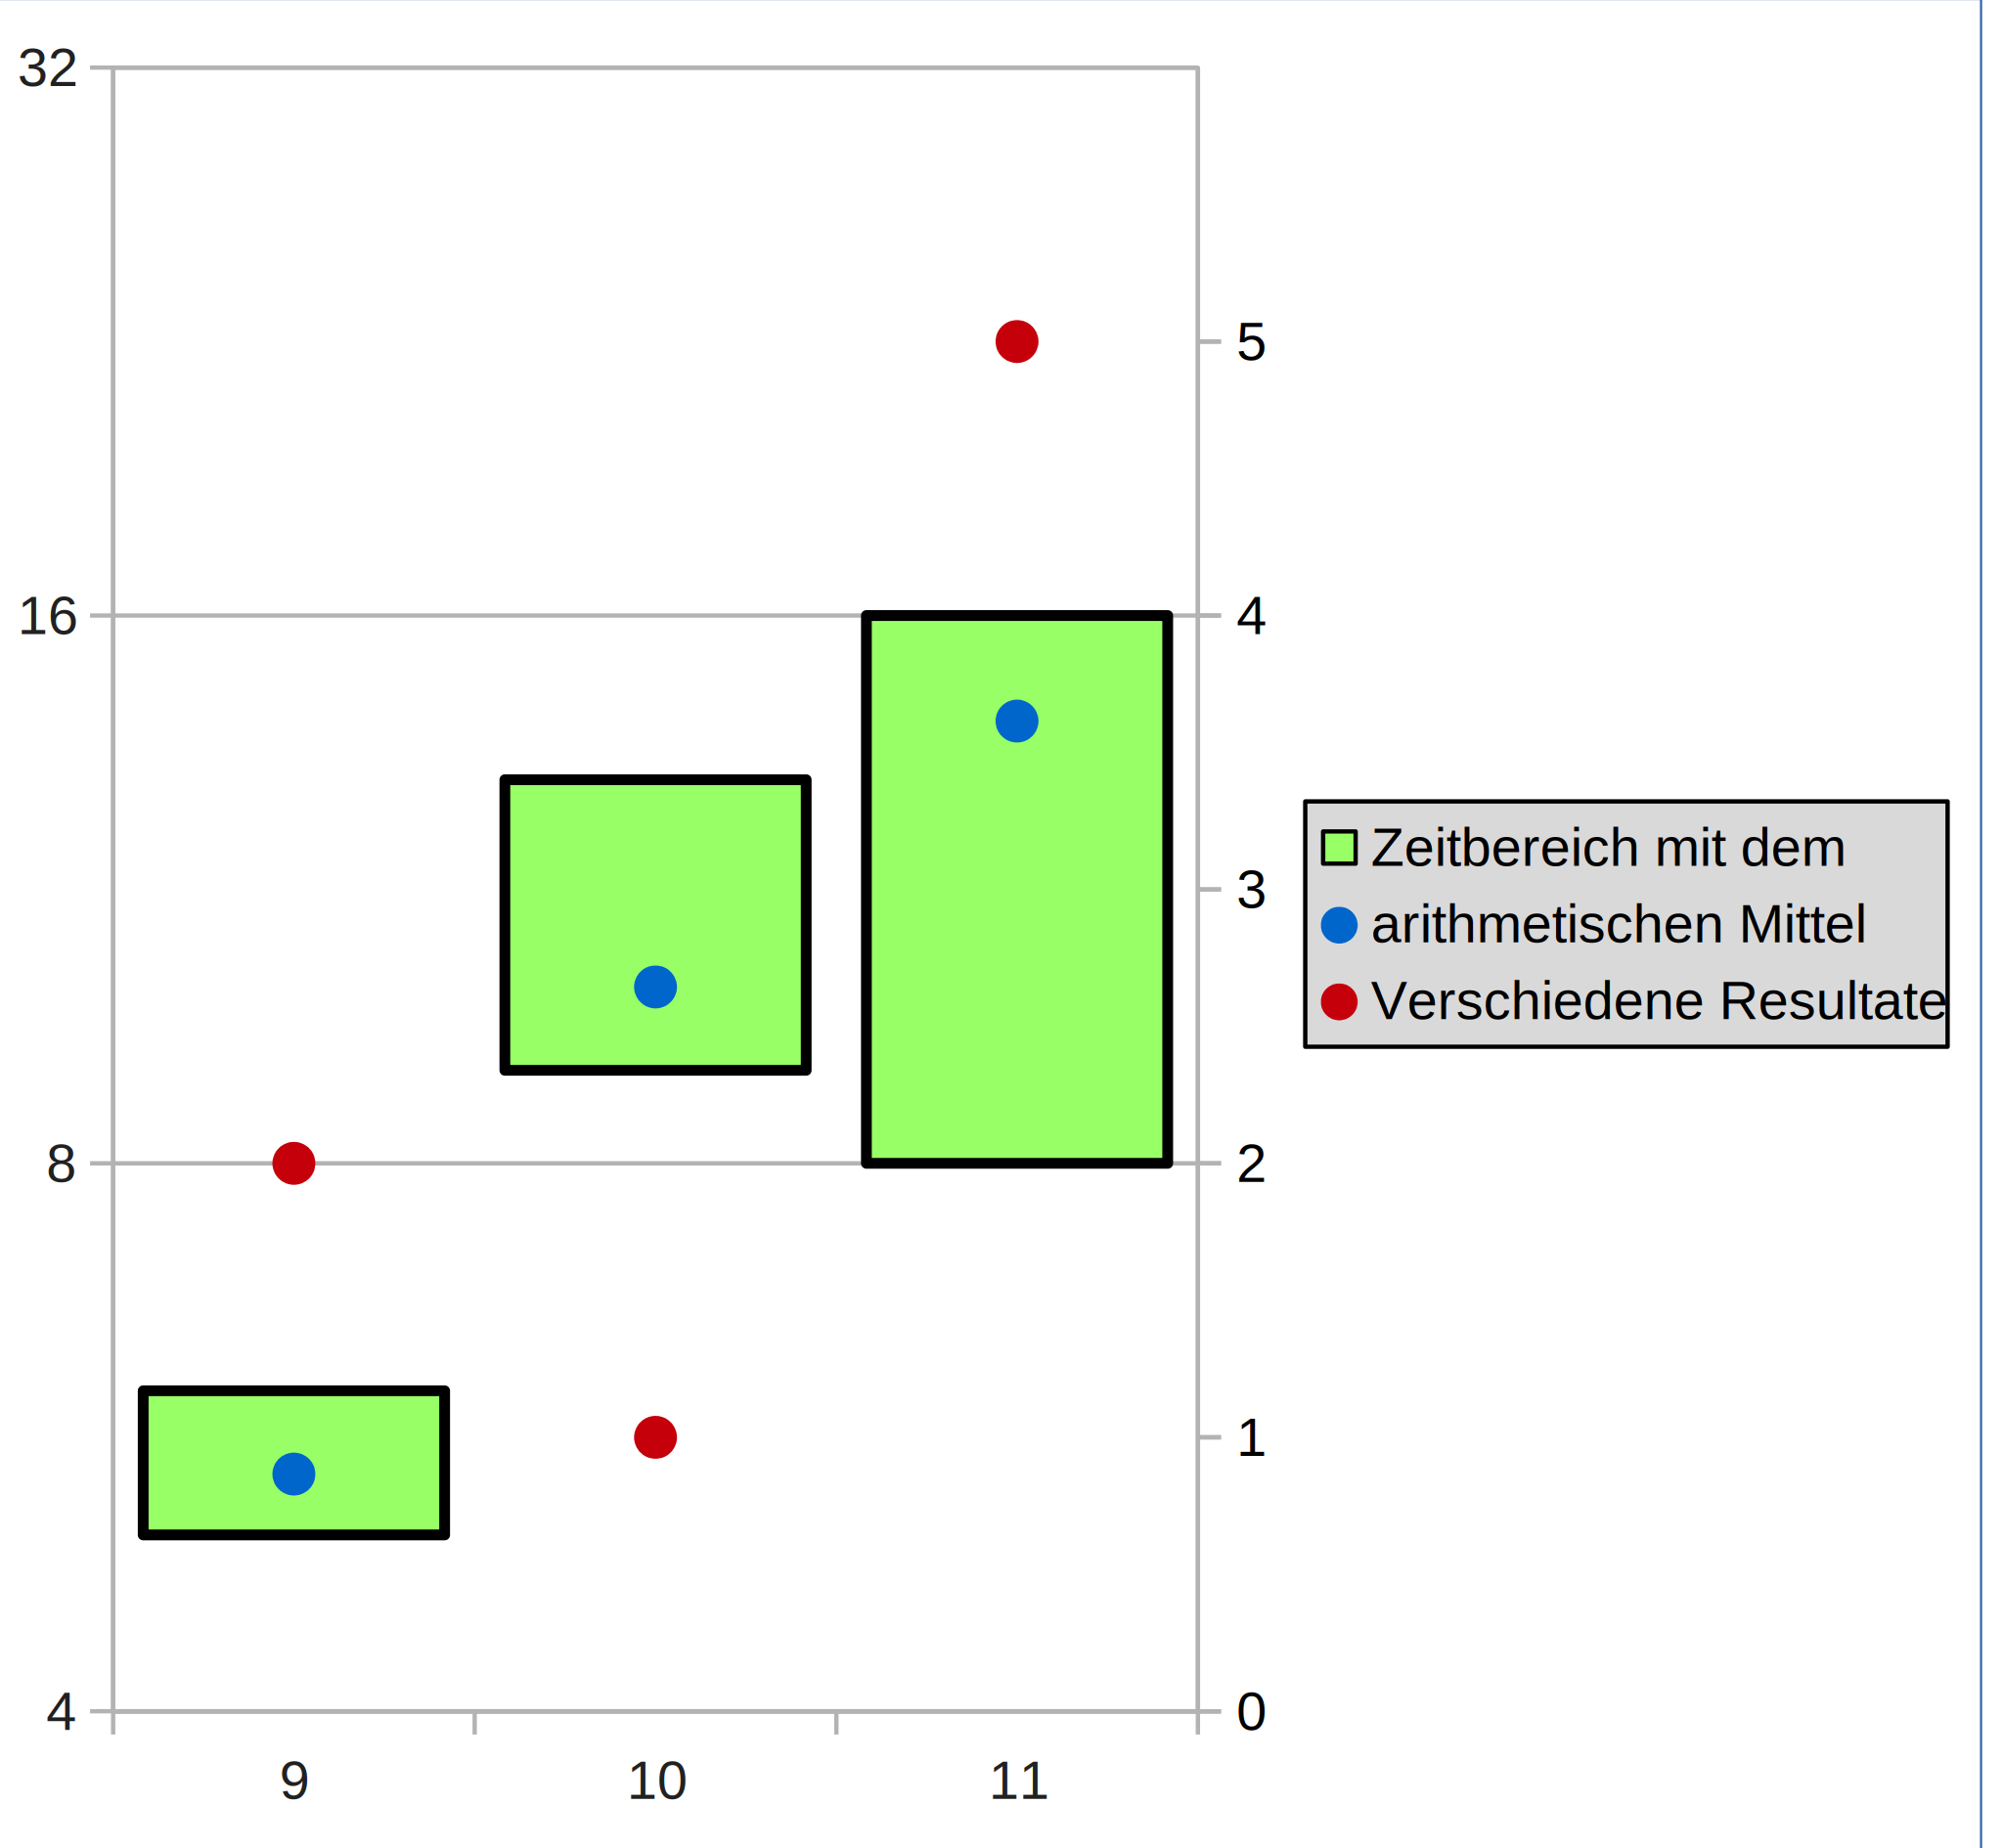
\includegraphics[scale=0.55]{images/data_legend}
  \caption{TODO}
  \label{fig:data_lengede}
\end{figure}

\section{Test ohne zusätzlich Klauseln als Bewertungsgrundlage}

\TODO{erledigen}
\section{Test mit modulinternen Klauseln}

\TODO{erledigen}

\begin{figure}[!h]
  \centering
  \begin{minipage}[c]{0.45\textwidth}
  \begin{flushleft}Gesamtdauer ohne XOR: 91:28:43\end{flushleft}
  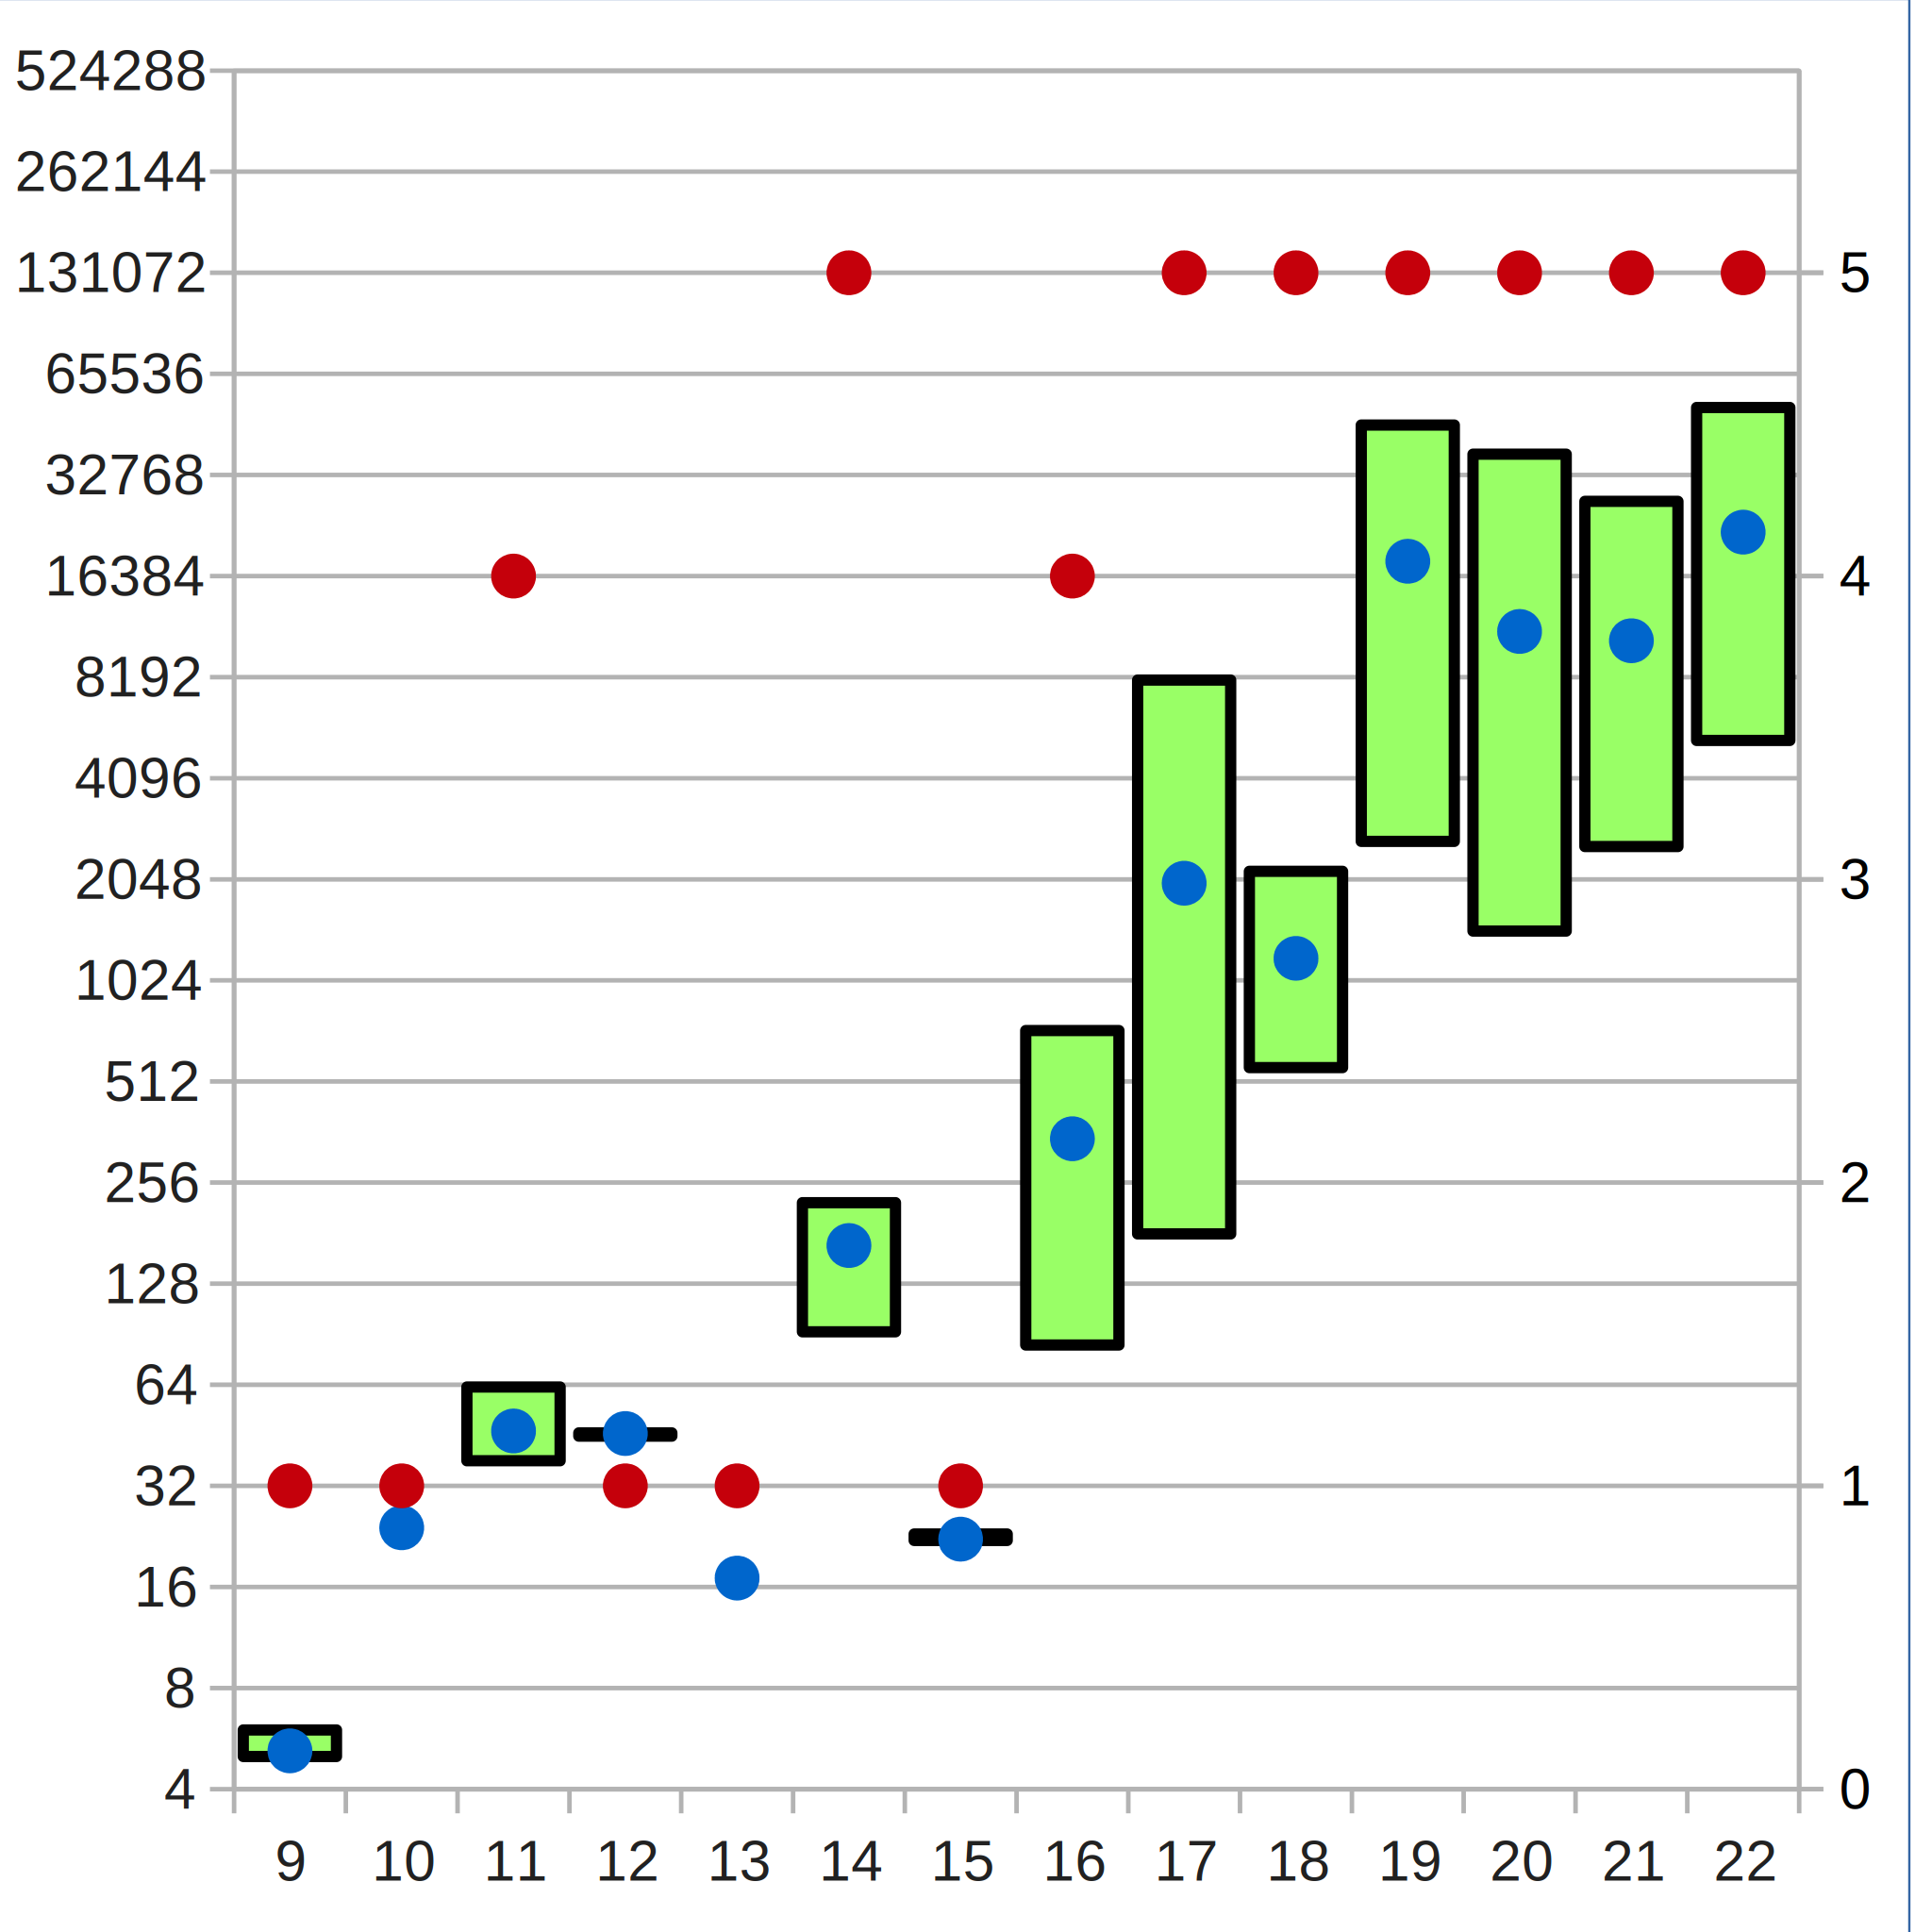
\includegraphics[scale=0.55]{images/data_modul_knf}
  \end{minipage}
  \begin{minipage}[c]{0.09\textwidth}
  ~~
  \end{minipage}
  \begin{minipage}[c]{0.45\textwidth}
  \begin{flushleft}Gesamtdauer mit XOR: 69:07:57\end{flushleft}
  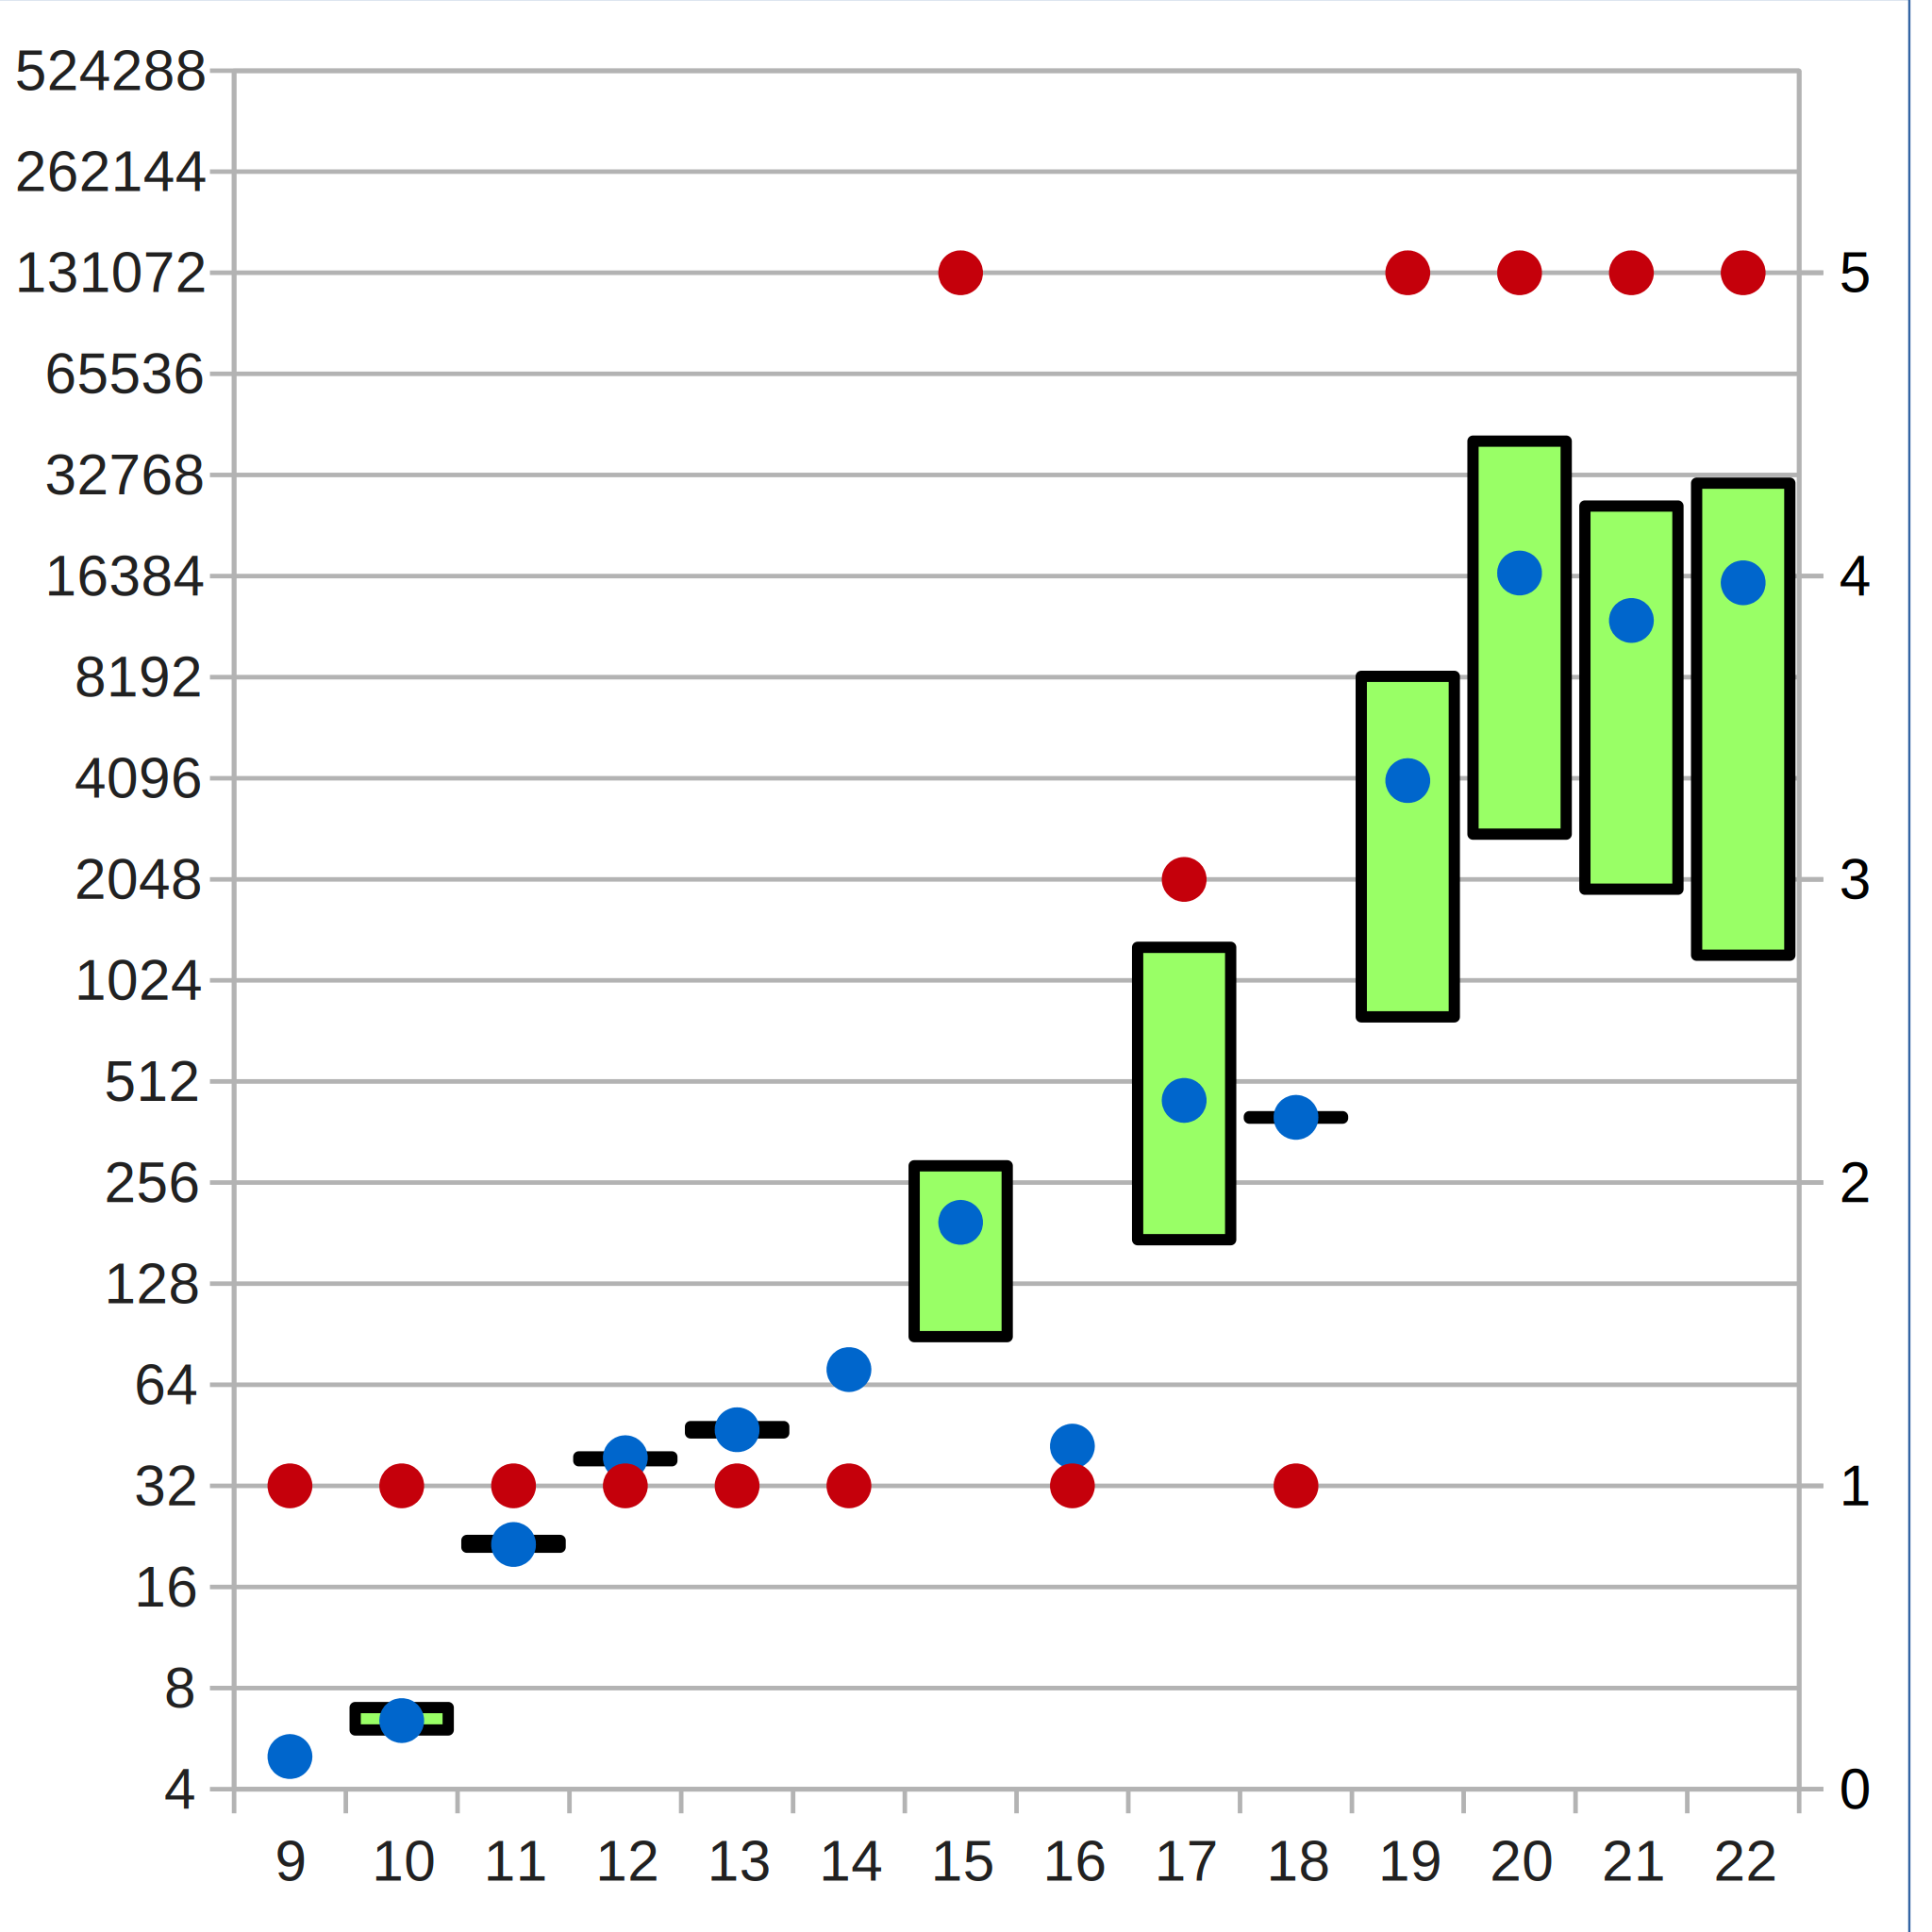
\includegraphics[scale=0.55]{images/data_modul_xor}
  \end{minipage}
  \caption{TODO}
  \label{fig:data_modul}
\end{figure}
\section{Test mit Distanzklauseln}

\TODO{erledigen}

\begin{figure}[!h]
  \centering
  \begin{minipage}[c]{0.45\textwidth}
  \begin{flushleft}Gesamtdauer ohne XOR: 155:31:37\end{flushleft}
  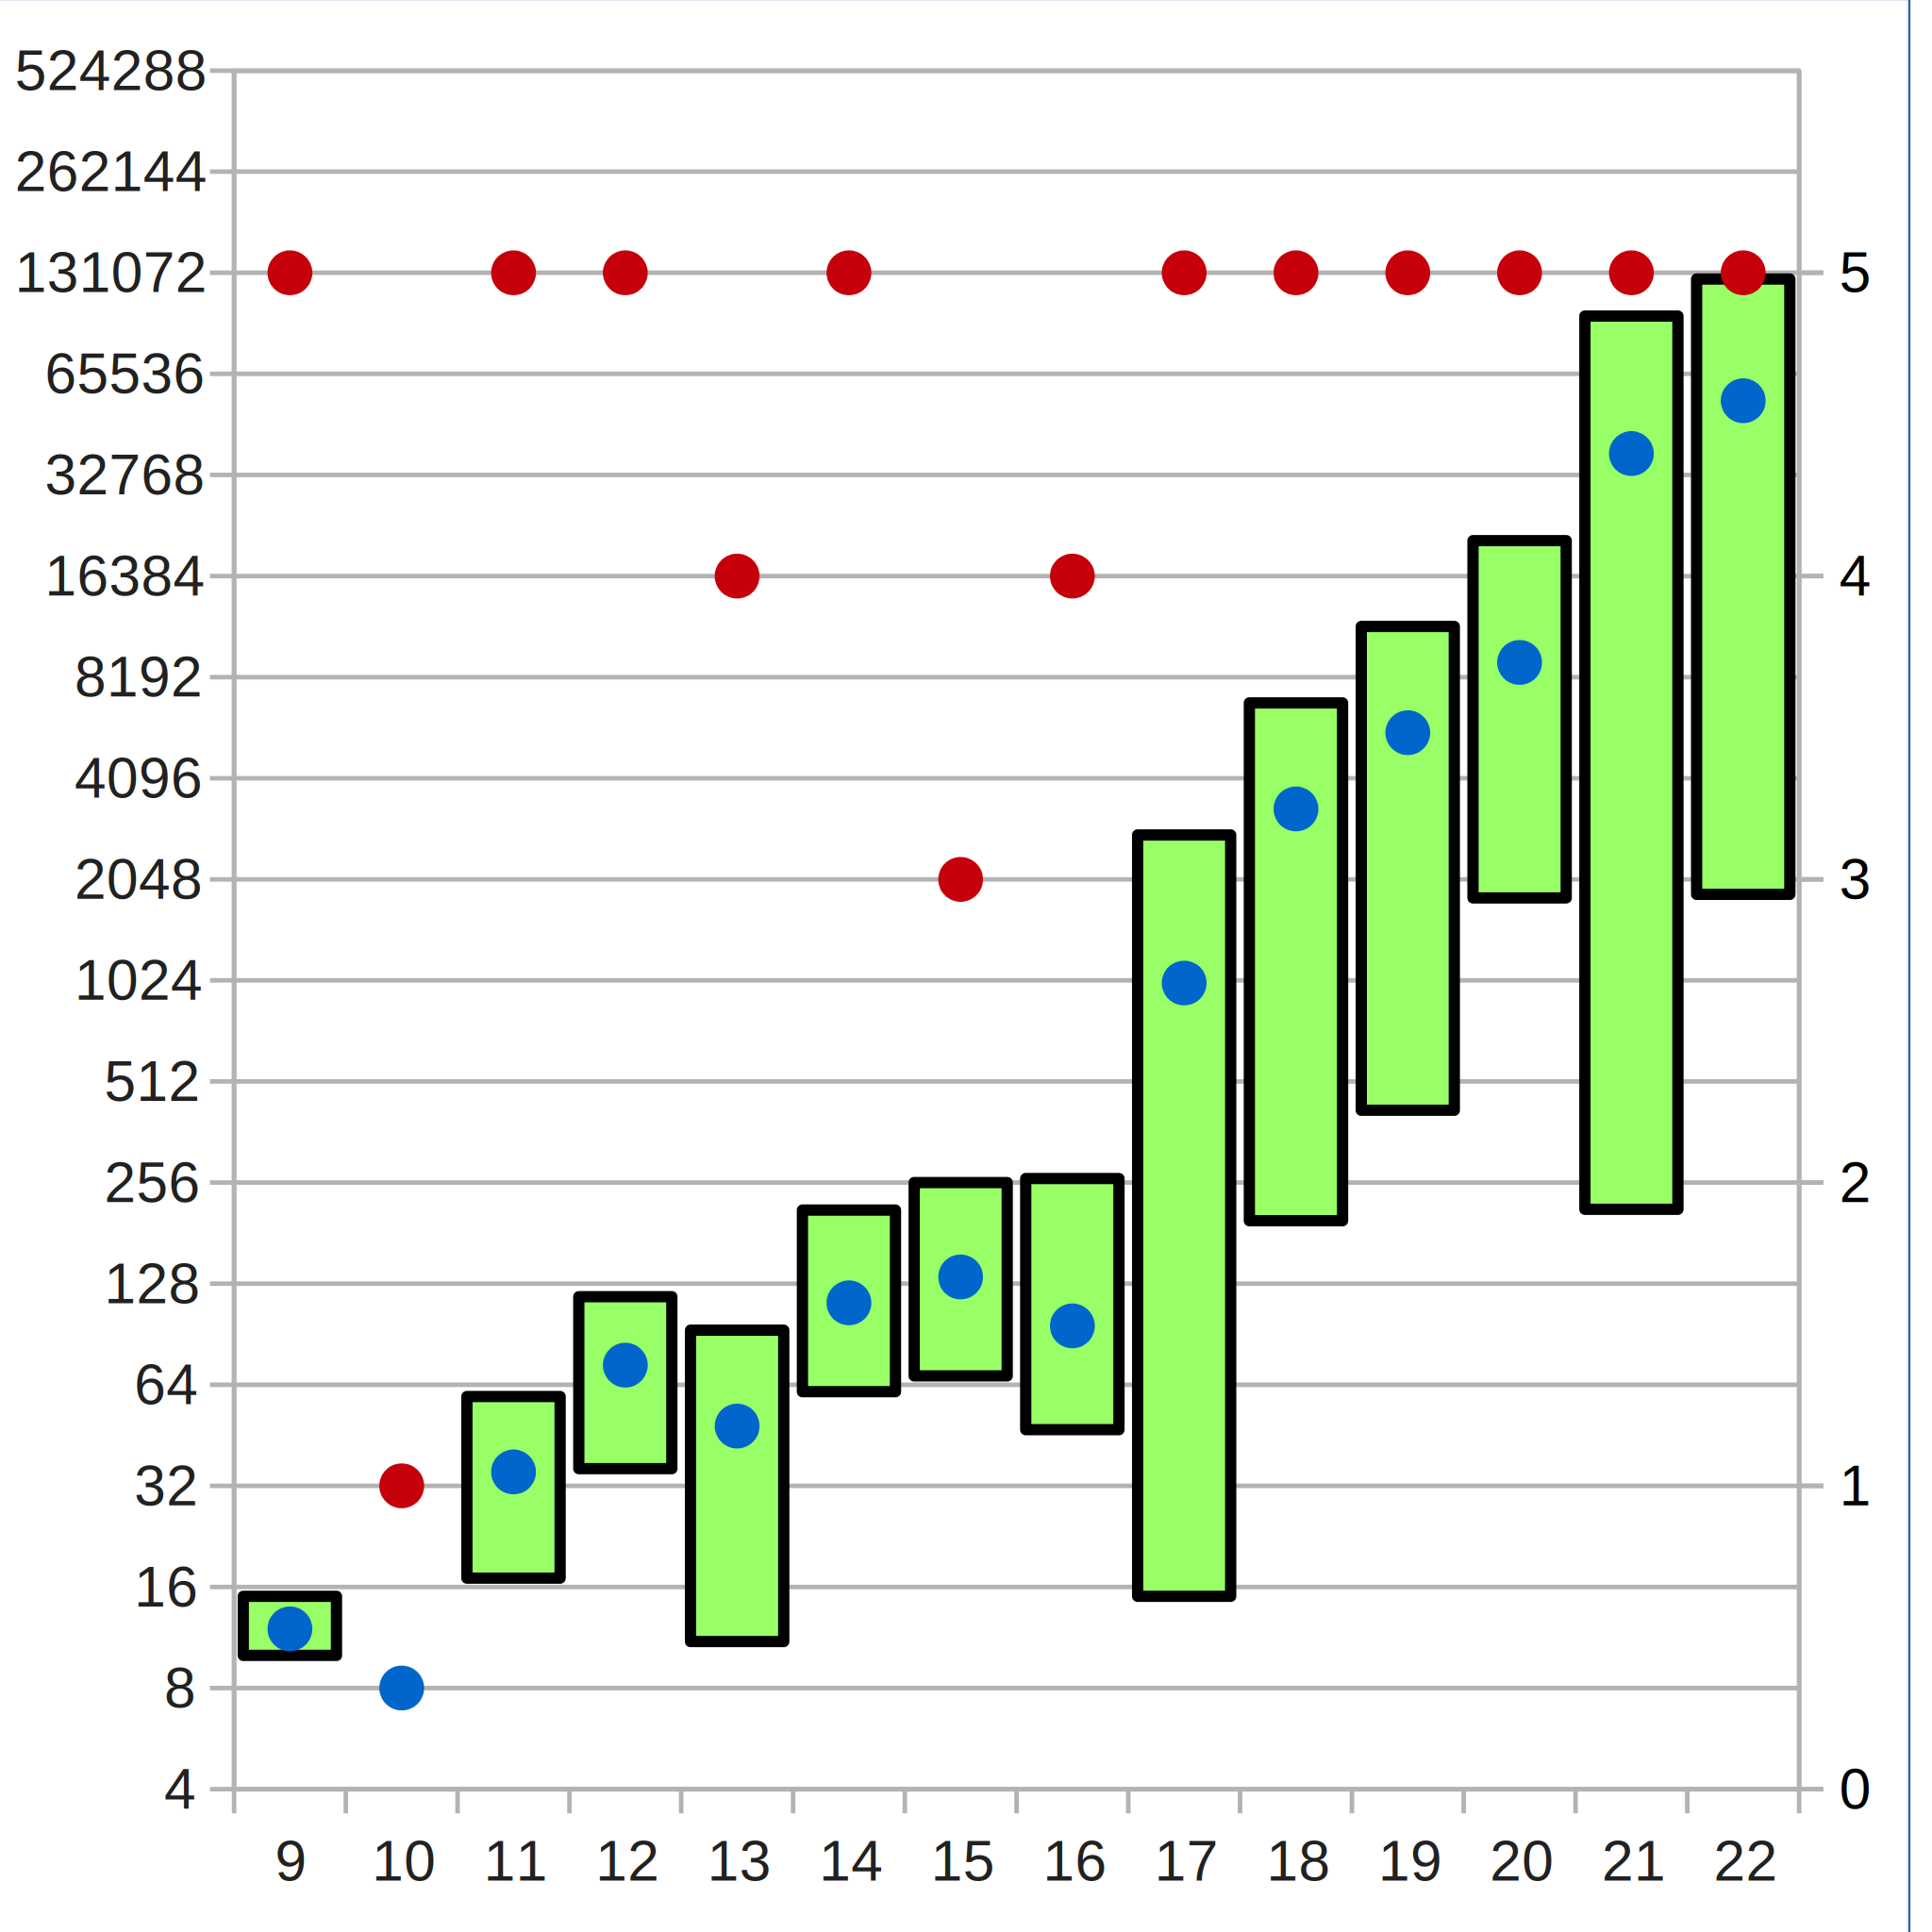
\includegraphics[scale=0.55]{images/data_dist_knf}
  \end{minipage}
  \begin{minipage}[c]{0.09\textwidth}
  ~~
  \end{minipage}
  \begin{minipage}[c]{0.45\textwidth}
  \begin{flushleft}Gesamtdauer mit XOR: 141:34:35\end{flushleft}
  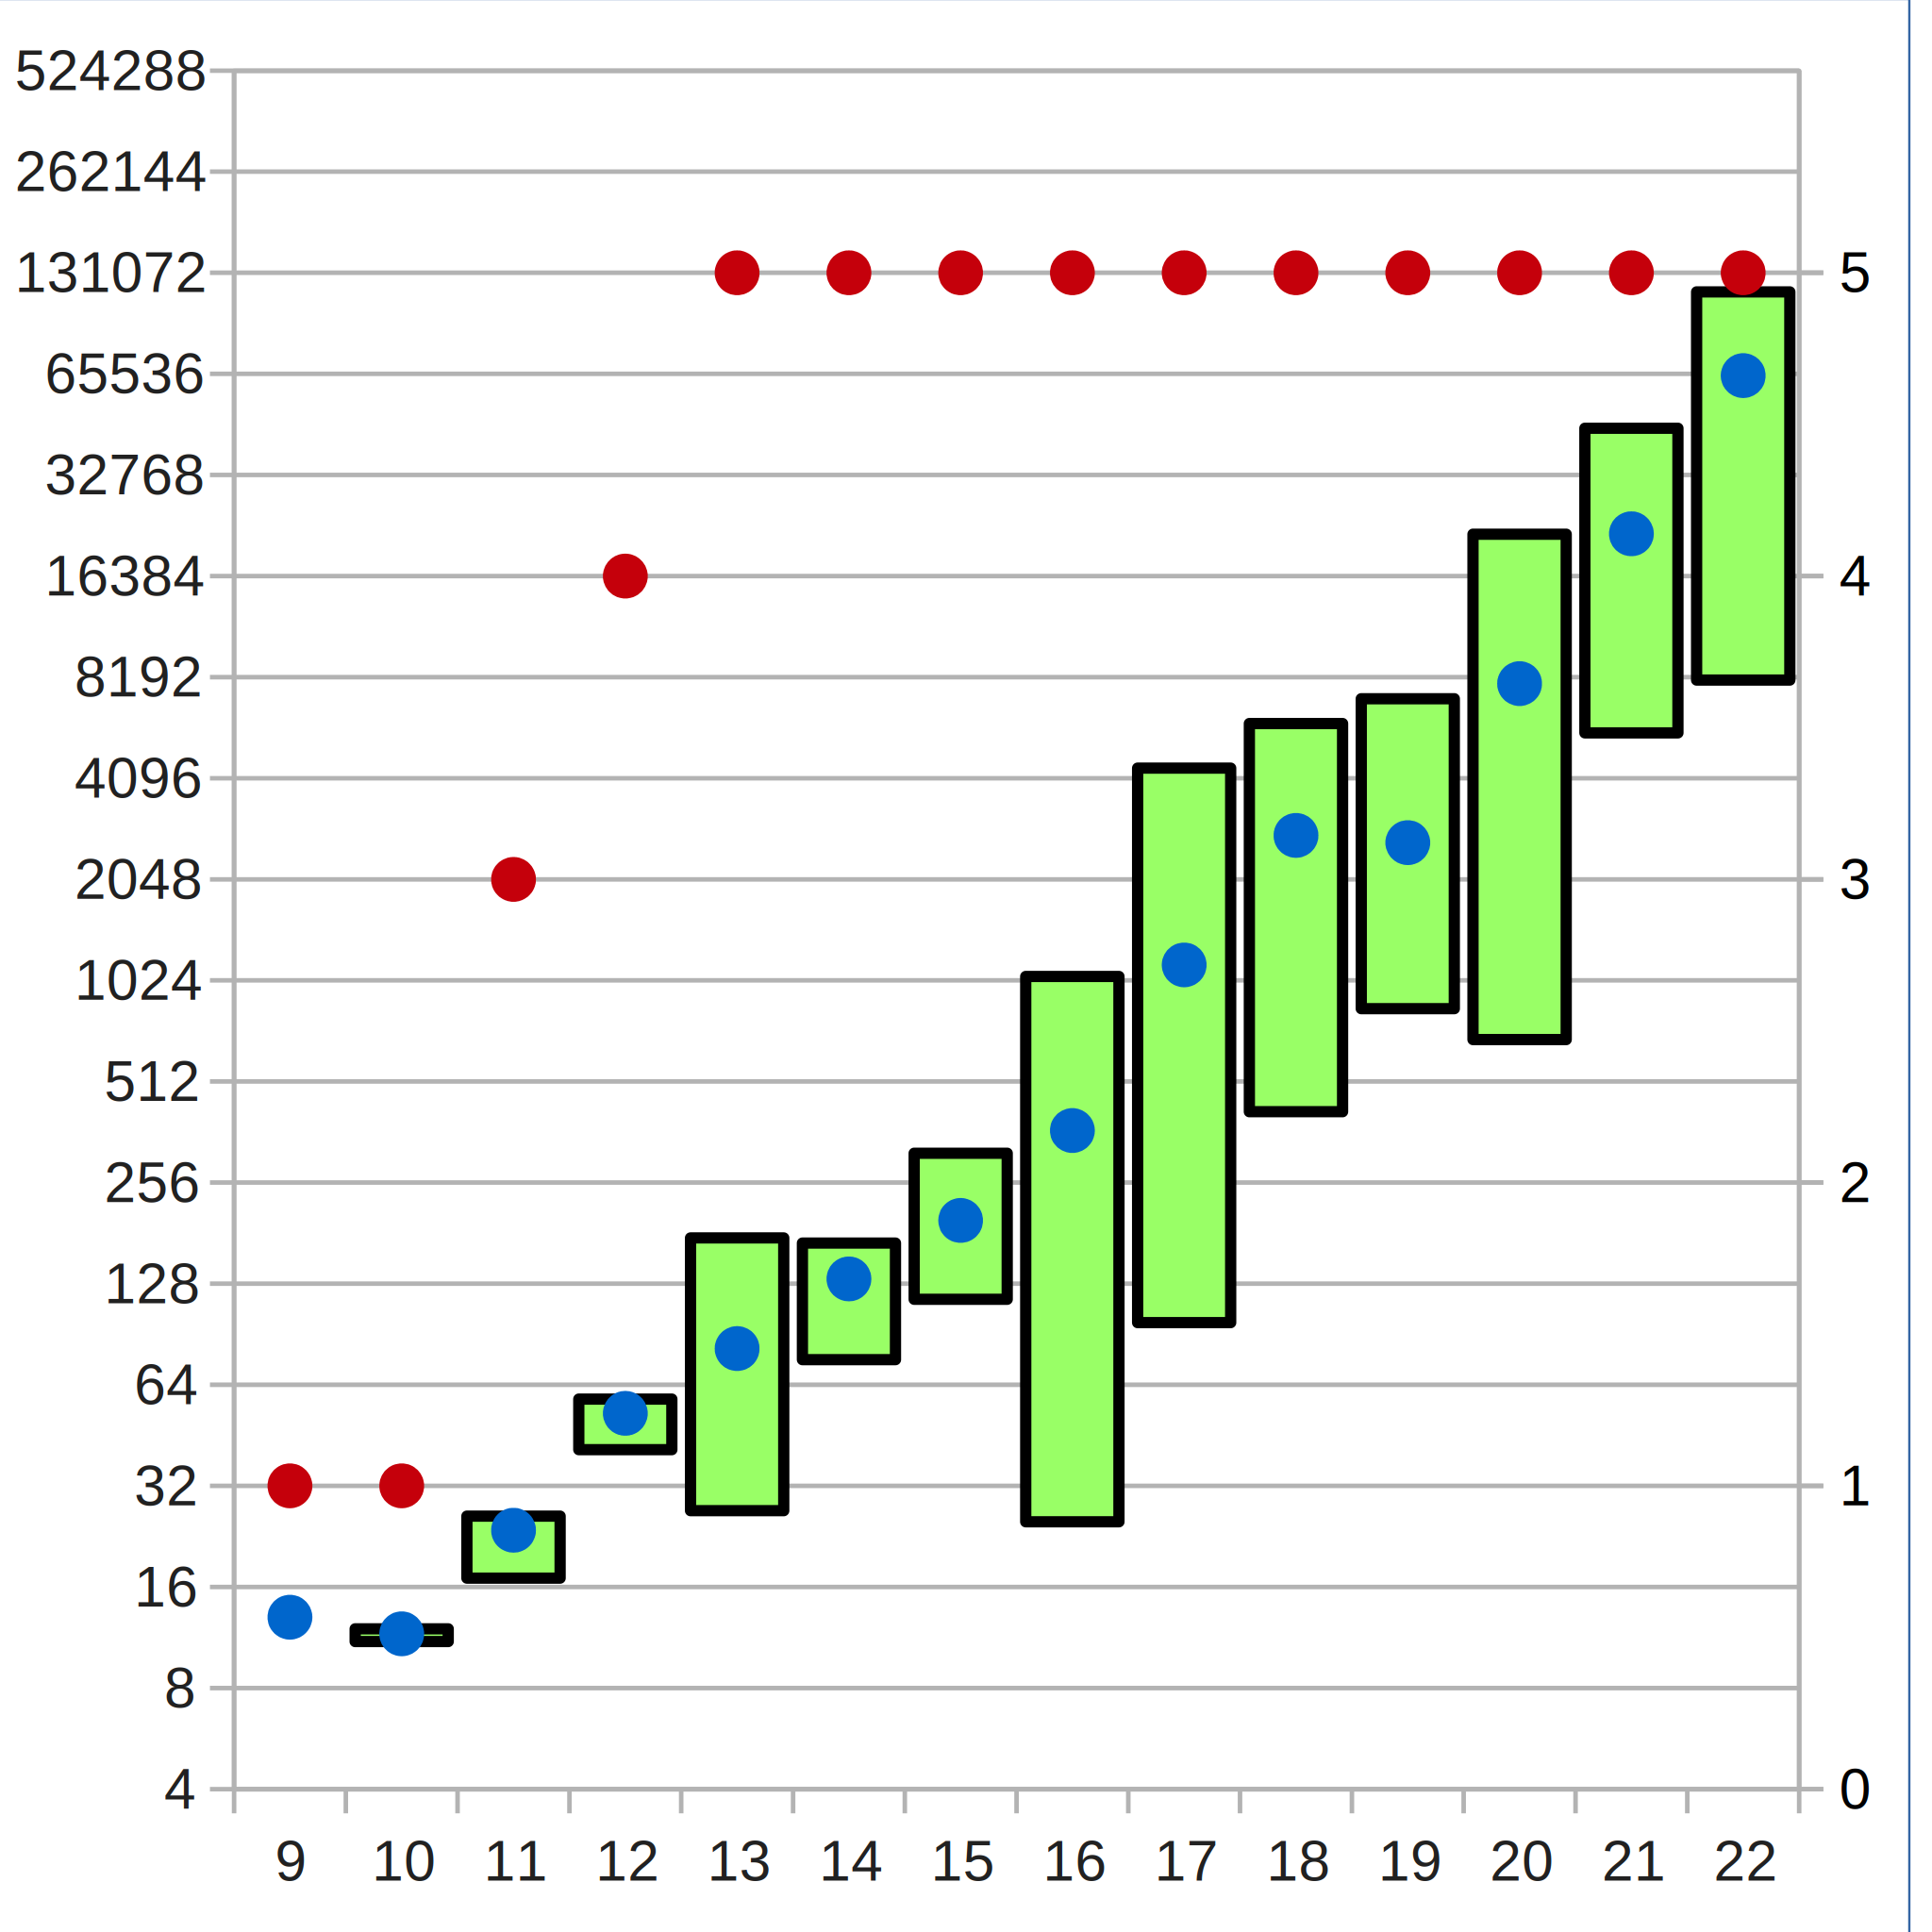
\includegraphics[scale=0.55]{images/data_dist_xor}
  \end{minipage}
  \caption{TODO}
  \label{fig:data_dist}
\end{figure}
\section{Test mit zusätzlichen Addiererklauseln}

sinnvoll, da diese einen großteil ausmachen und den Sat-Solver ausbremsen könnten?

\TODO{erledigen}

\begin{figure}[!h]
  \centering
  \begin{minipage}[c]{0.45\textwidth}
  \begin{flushleft}Gesamtdauer ohne XOR: 410:59:52\end{flushleft}
  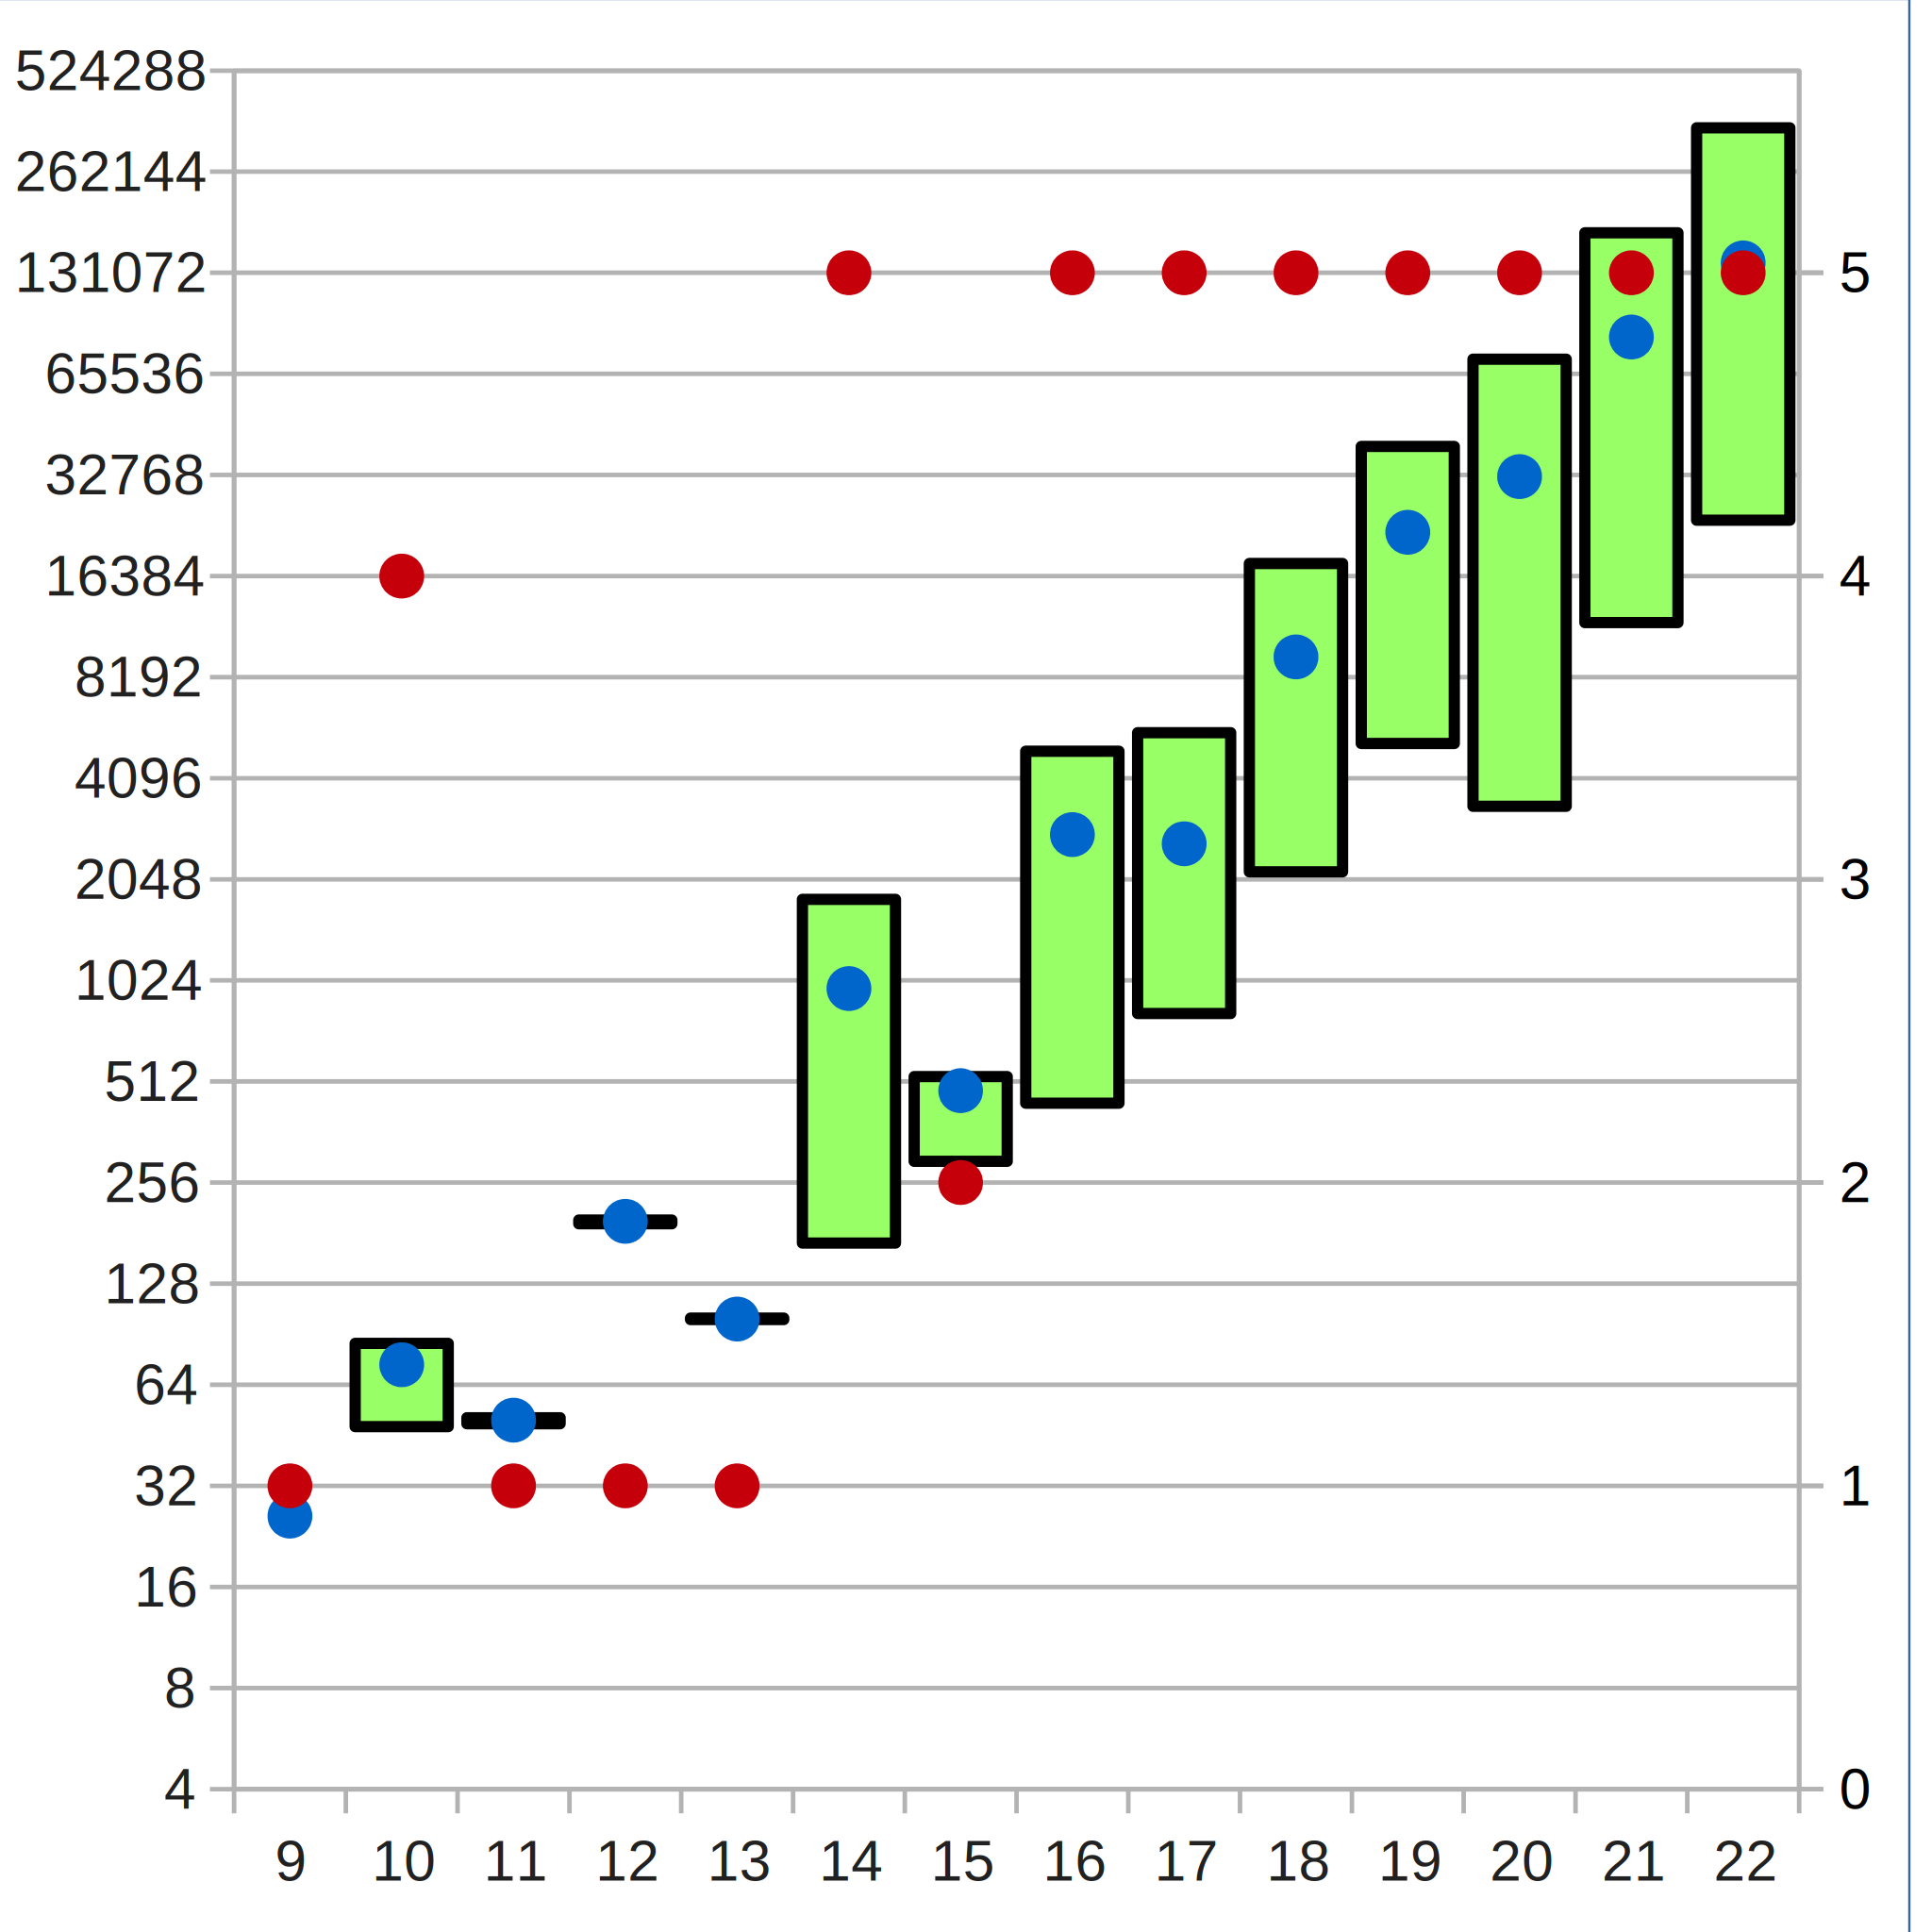
\includegraphics[scale=0.55]{images/data_add_knf}
  \end{minipage}
  \begin{minipage}[c]{0.09\textwidth}
  ~~
  \end{minipage}
  \begin{minipage}[c]{0.45\textwidth}
  \begin{flushleft}Gesamtdauer mit XOR: 491:53:48\end{flushleft}
  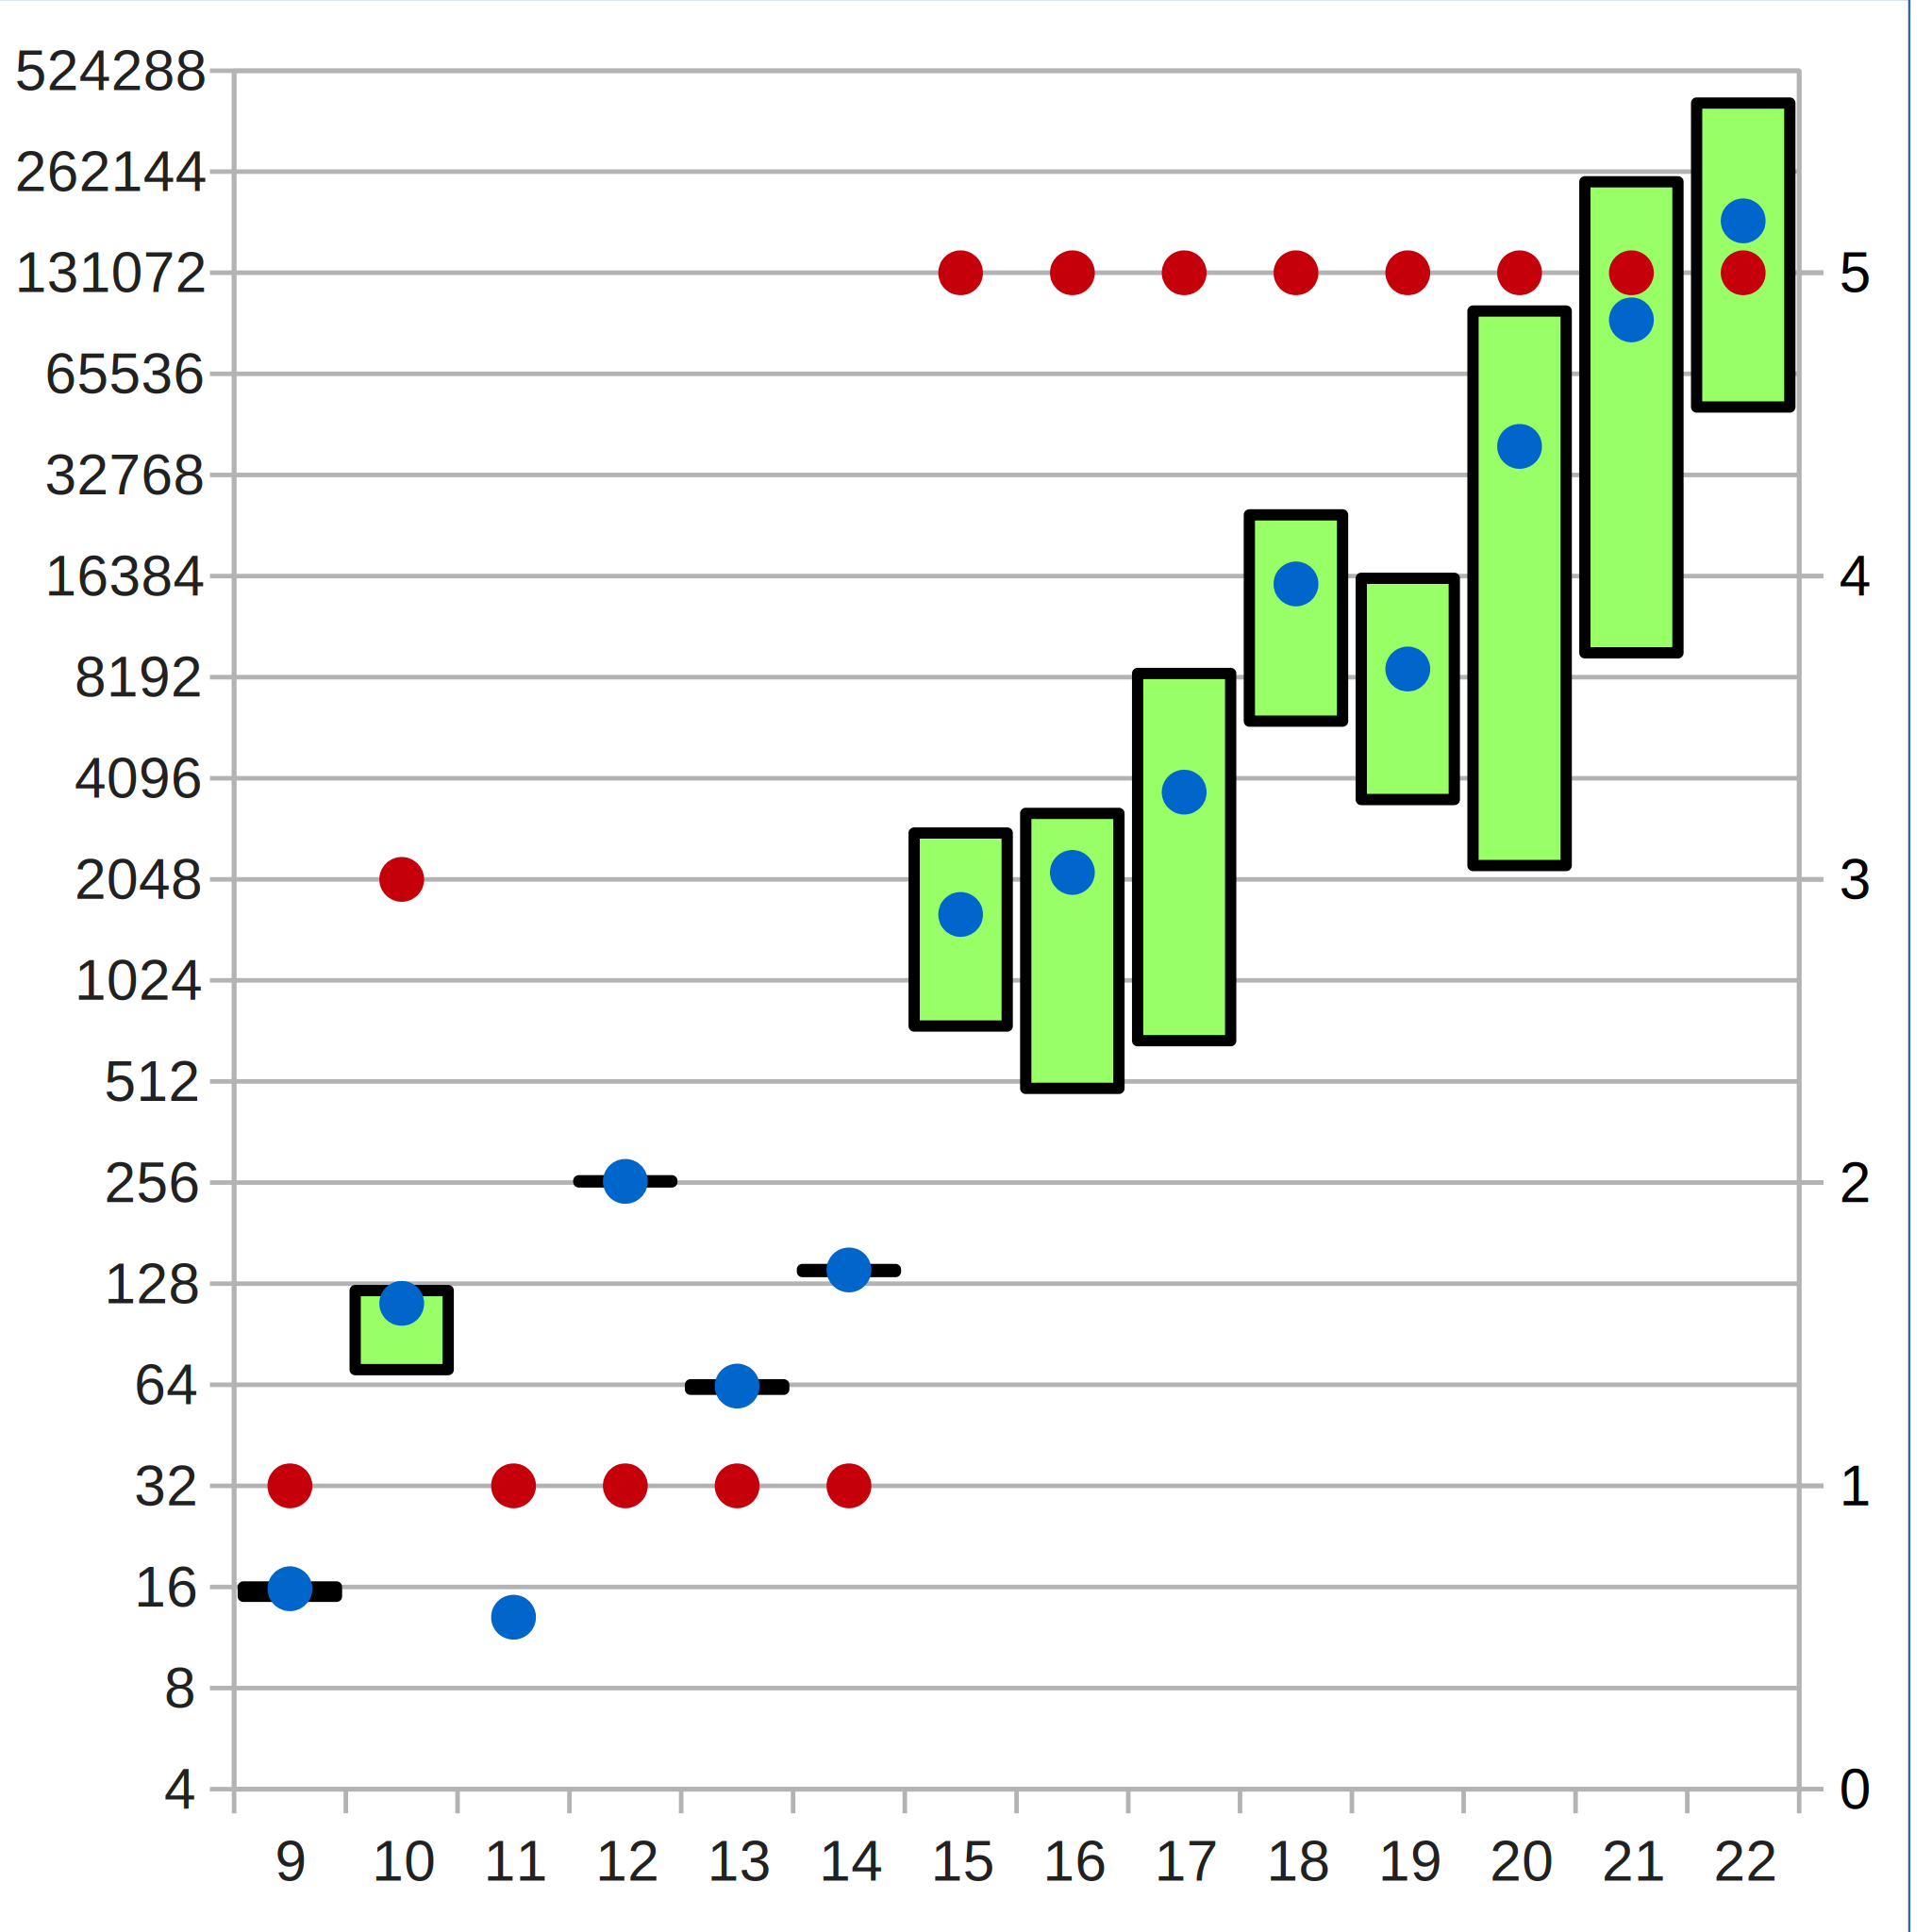
\includegraphics[scale=0.55]{images/data_add_xor}
  \end{minipage}
  \caption{TODO}
  \label{fig:data_add}
\end{figure}
\section{Test mit zusätzlichem Wissen}

In Abschnitt \ref{sec:ana:rundenfunktion} wurde wissen beschrieben\\
test mit diesem wissen

mehr literale

subtraktion ergänzen

\TODO{erledigen}

\begin{figure}[!h]
  \centering
  \begin{minipage}[c]{0.45\textwidth}
  \begin{flushleft}Gesamtdauer ohne XOR: 205:09:48\end{flushleft}
  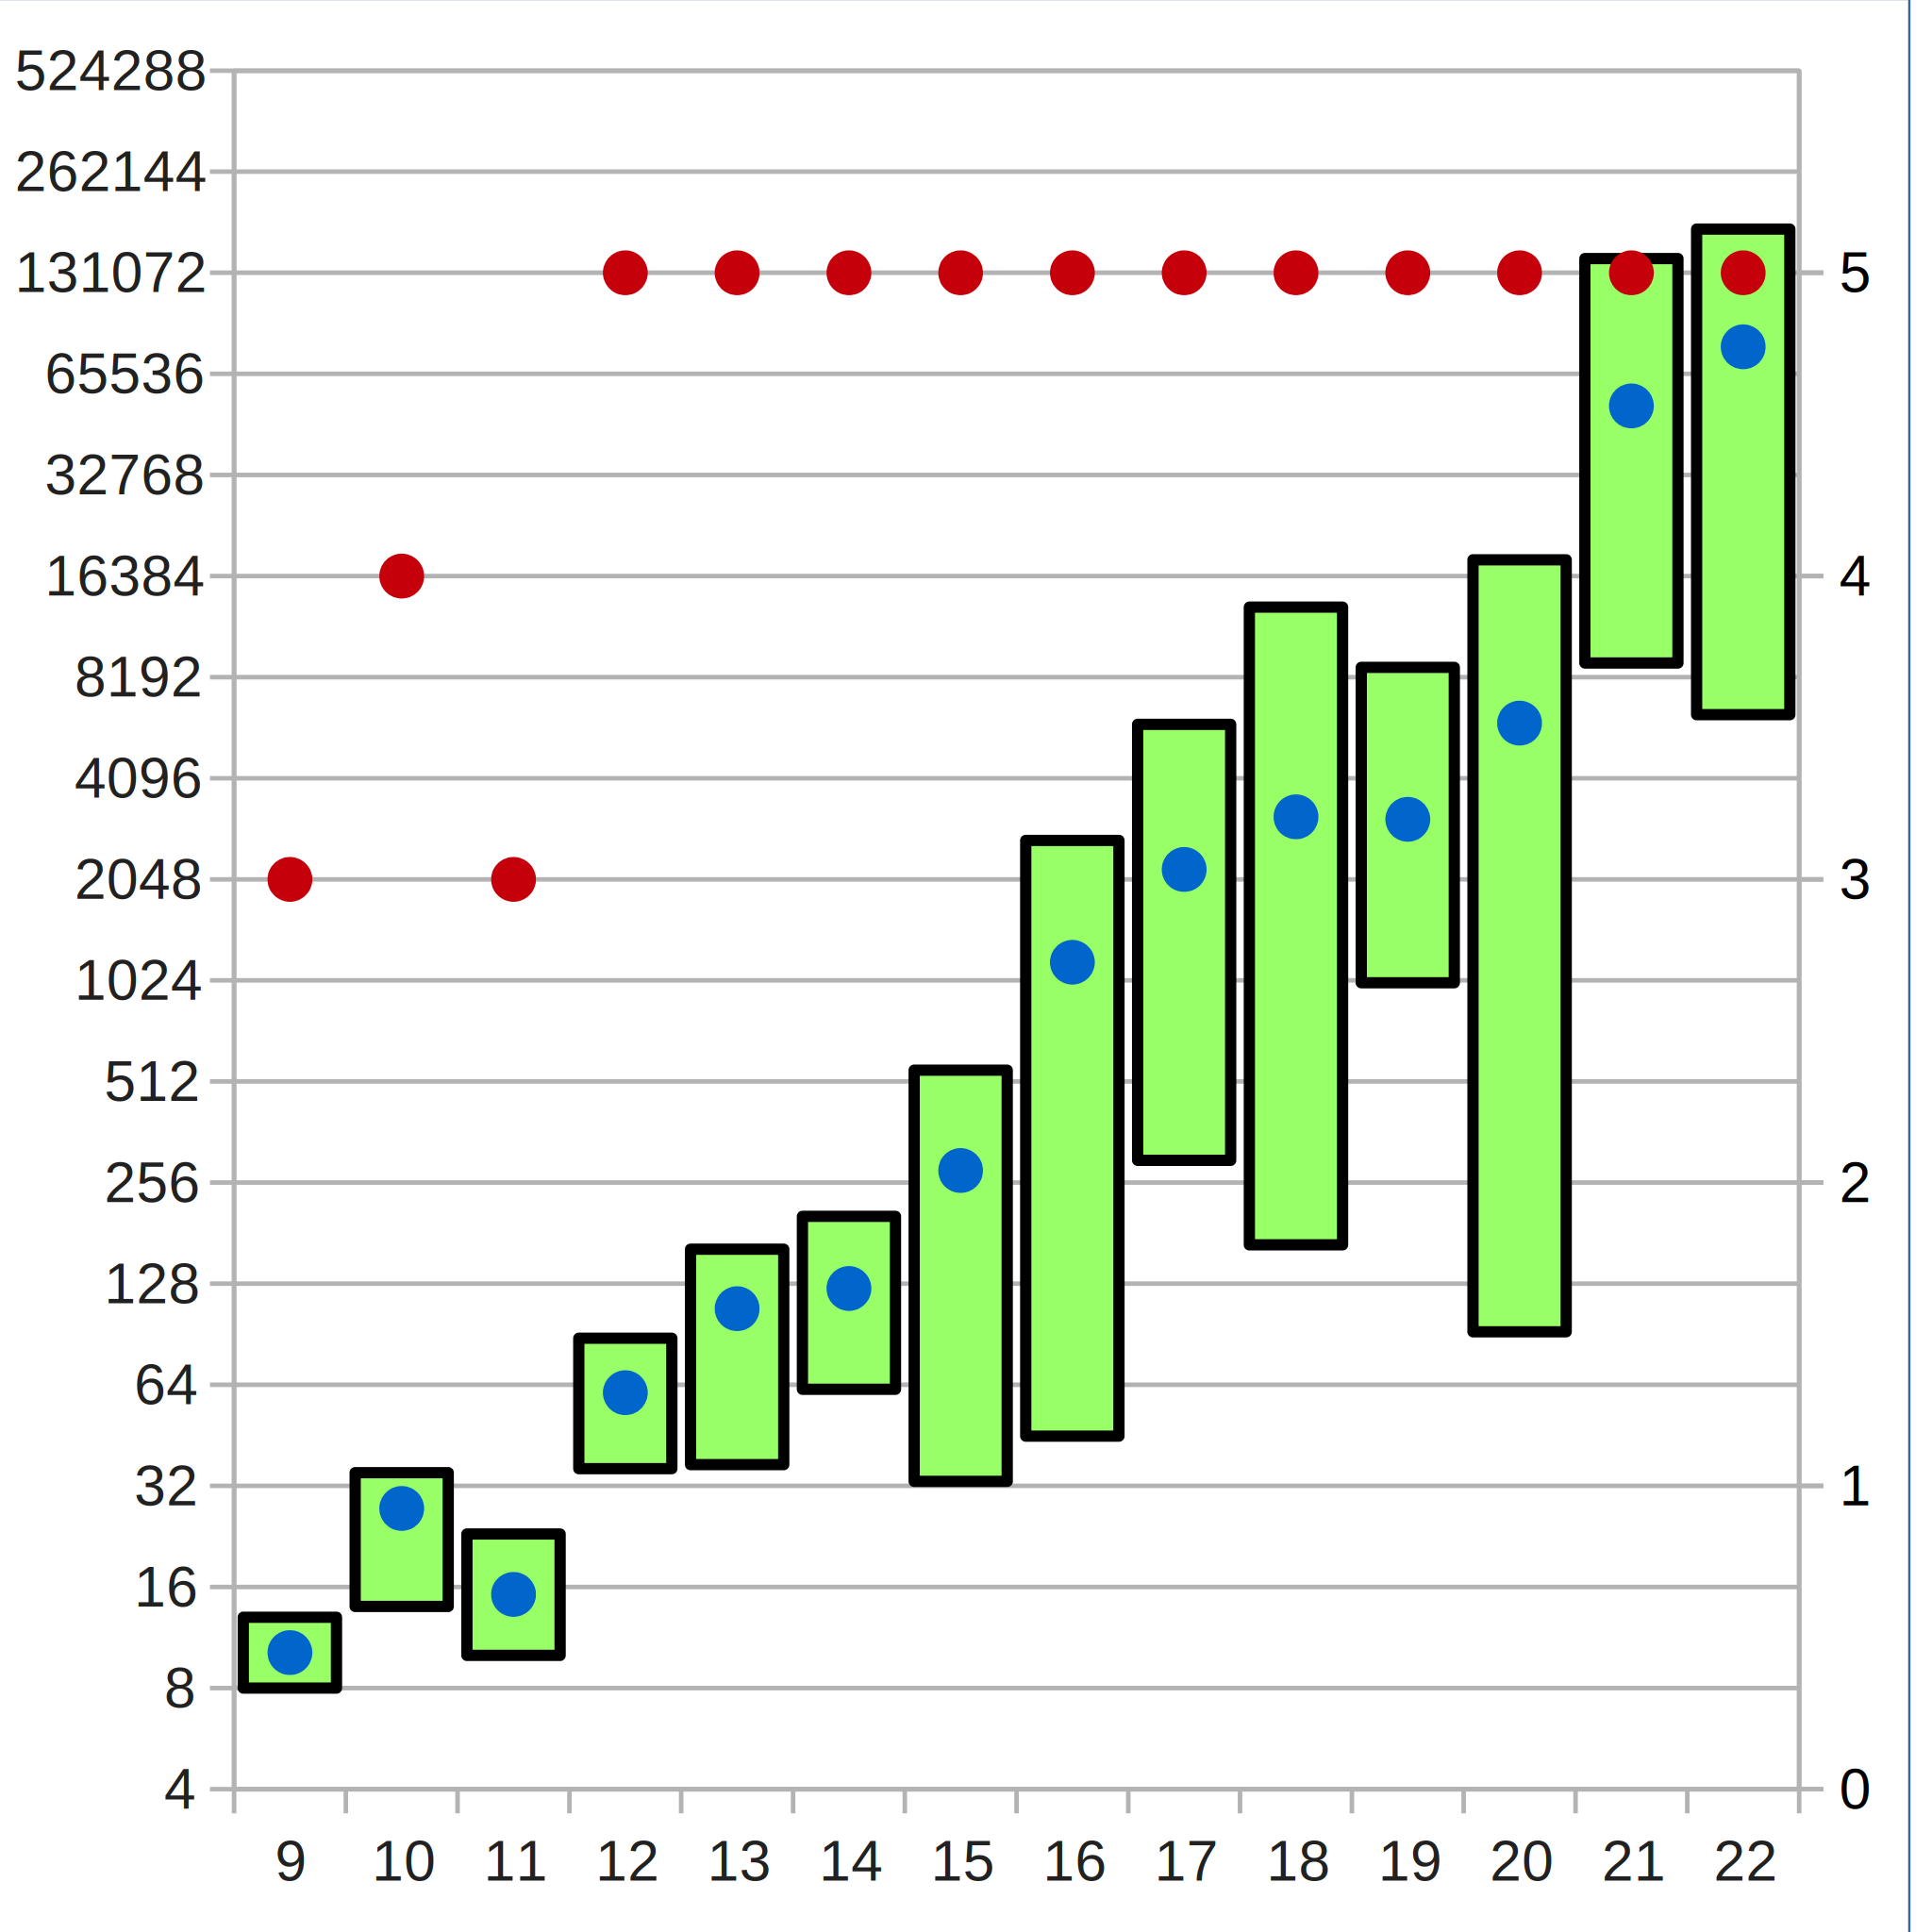
\includegraphics[scale=0.55]{images/data_know_knf}
  \end{minipage}
  \begin{minipage}[c]{0.09\textwidth}
  ~~
  \end{minipage}
  \begin{minipage}[c]{0.45\textwidth}
  \begin{flushleft}Gesamtdauer mit XOR: 100:41:09\end{flushleft}
  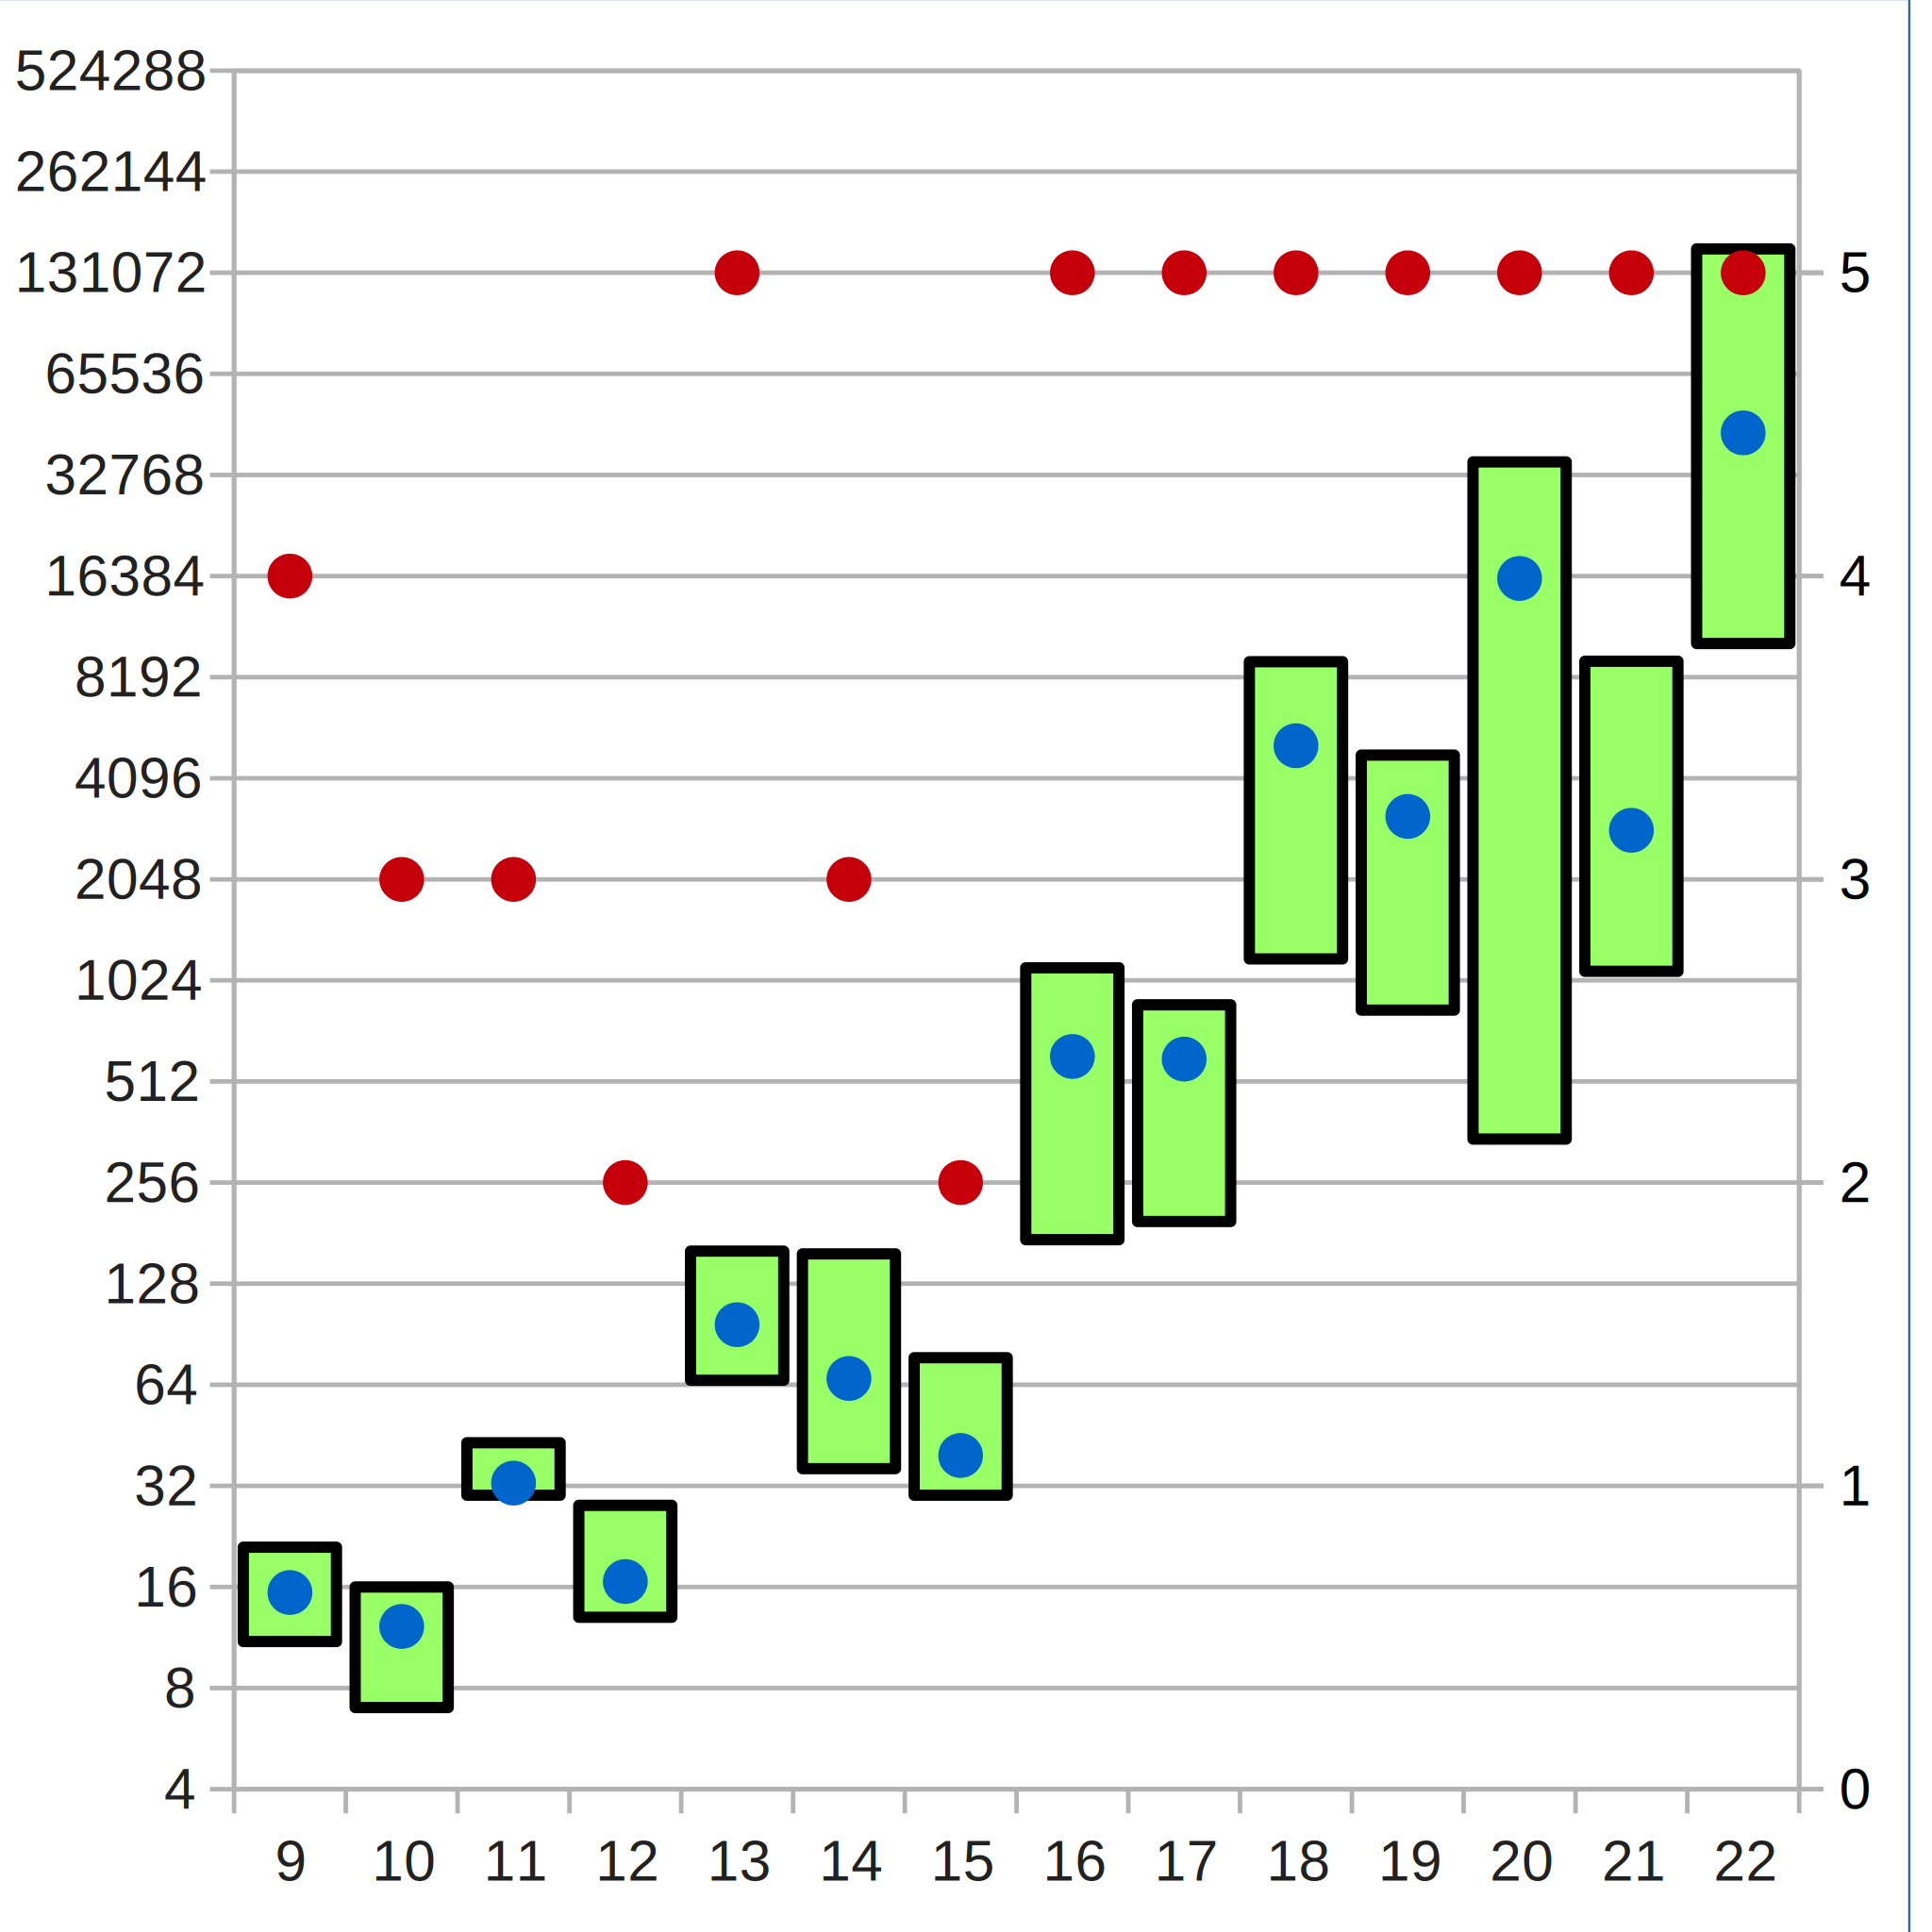
\includegraphics[scale=0.55]{images/data_know_xor}
  \end{minipage}
  \caption{TODO}
  \label{fig:data_know}
\end{figure}
\section{Test mit allen vorteilhaften Klauseln}

\TODO{erledigen}

\begin{figure}[!h]
  \centering
  \begin{minipage}[c]{0.45\textwidth}
  \begin{flushleft}Gesamtdauer ohne XOR: 224:36:00\end{flushleft}
  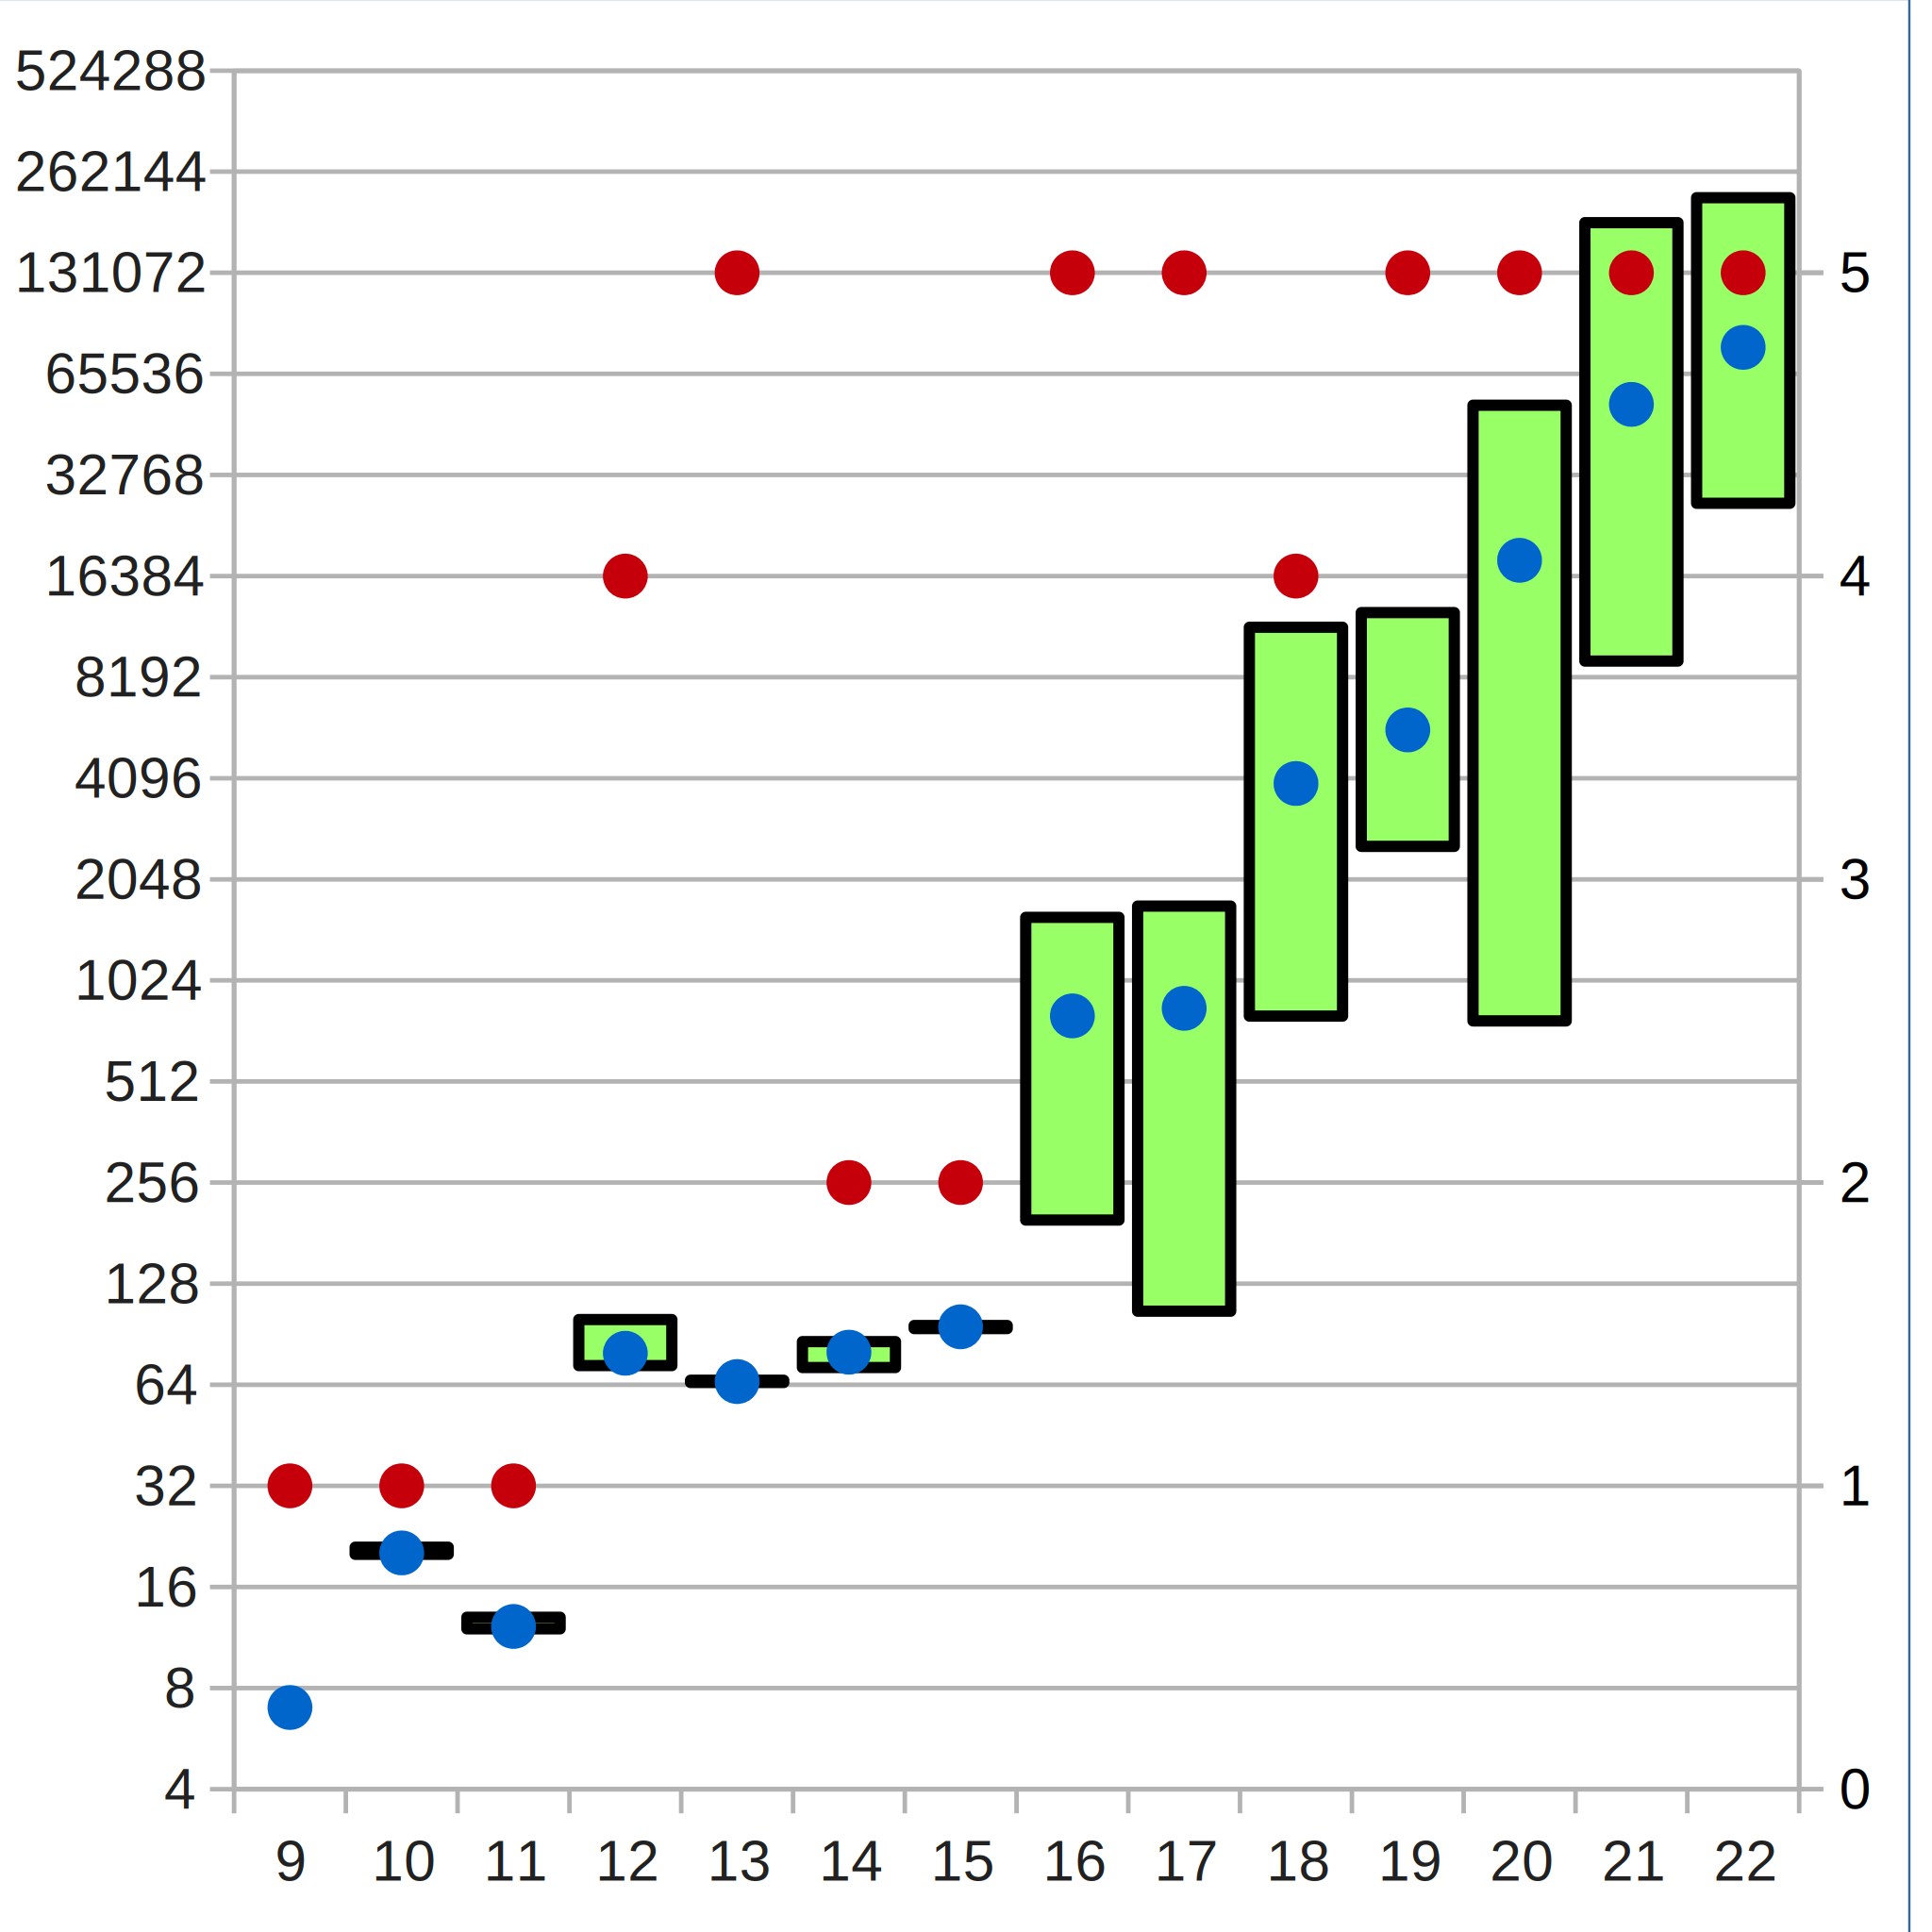
\includegraphics[scale=0.55]{images/data_final_knf}
  \end{minipage}
  \begin{minipage}[c]{0.09\textwidth}
  ~~
  \end{minipage}
  \begin{minipage}[c]{0.45\textwidth}
  \begin{flushleft}Gesamtdauer mit XOR: 136:37:46\end{flushleft}
  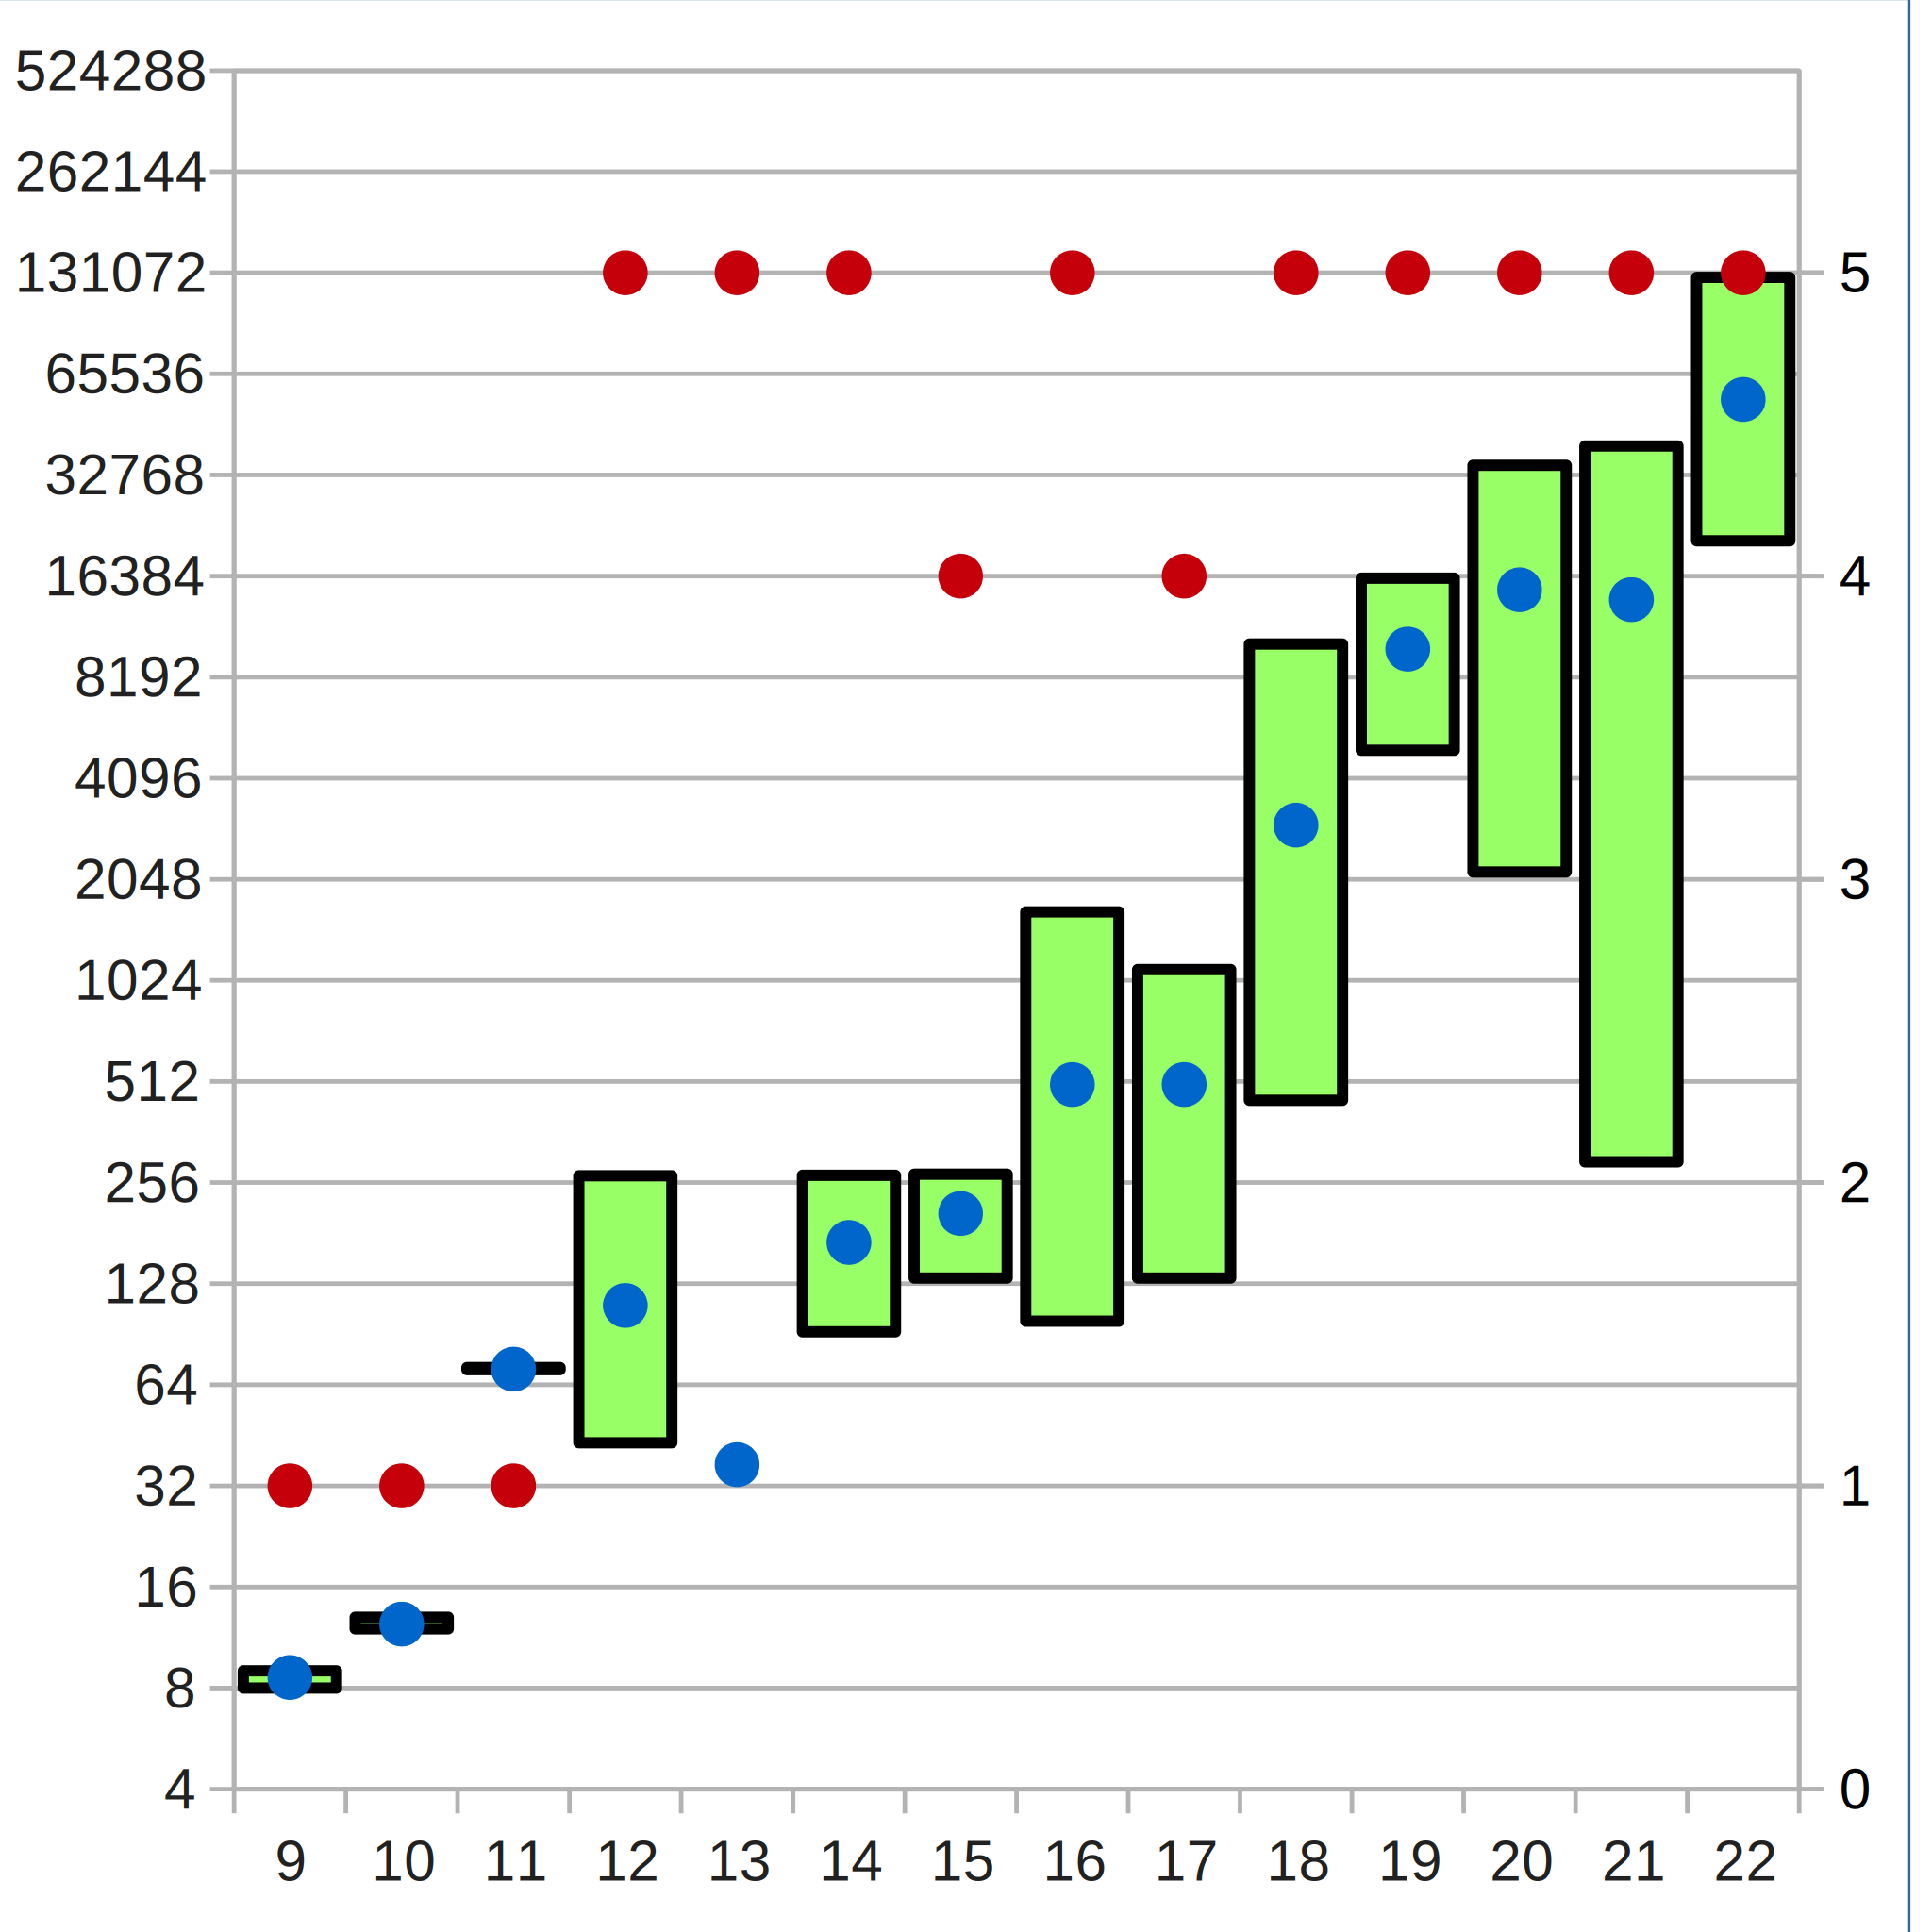
\includegraphics[scale=0.55]{images/data_final_xor}
  \end{minipage}
  \caption{TODO}
  \label{fig:data_final}
\end{figure}
\section{Vergleich mit CBMC}

\TODO{erledigen}